\documentclass[aspectratio=169,11pt]{beamer}

\usepackage[T1]{fontenc}
\usepackage{lmodern}
\usepackage{amsmath,amssymb}
\usepackage{tikz}
\usetikzlibrary{arrows.meta,positioning,calc}
\graphicspath{{frontend/ops/dss/benchmark/}{../frontend/ops/dss/benchmark/}}

\definecolor{ink}{HTML}{17324D}
\definecolor{teal}{HTML}{00878A}
\definecolor{blue}{HTML}{347AB8}
\definecolor{orange}{HTML}{D77A43}
\definecolor{muted}{HTML}{617385}
\definecolor{pale}{HTML}{EEF5F8}

\setbeamercolor{normal text}{fg=ink,bg=white}
\setbeamercolor{frametitle}{fg=white,bg=ink}
\setbeamercolor{structure}{fg=teal}
\setbeamercolor{block title}{fg=white,bg=teal}
\setbeamercolor{block body}{fg=ink,bg=pale}
\setbeamertemplate{navigation symbols}{}
\setbeamertemplate{itemize item}{\color{teal}\small$\blacktriangleright$}
\setbeamertemplate{footline}{%
  \hfill\color{muted}\scriptsize SFEM \;|\; Cellwise matrix-free operators
  \hspace{0.7cm}\insertframenumber/\inserttotalframenumber\hspace{0.45cm}\vspace{0.18cm}}
\setbeamertemplate{frametitle}{%
  \nointerlineskip
  \begin{beamercolorbox}[wd=\paperwidth,ht=0.68cm,dp=0.23cm,leftskip=0.52cm]{frametitle}%
    \usebeamerfont{frametitle}\insertframetitle
  \end{beamercolorbox}}

\tikzset{
  flowbox/.style={draw=teal!75!black,fill=pale,rounded corners=3pt,
                  minimum width=2.2cm,minimum height=1.10cm,align=center,
                  font=\small,inner sep=4pt},
  flowarrow/.style={-{Stealth[length=3mm]},line width=1.2pt,draw=teal}
}

% One frame of a four-step walk through the fastest BXYZE index.
\newcommand{\bxyzelanestep}[1]{%
  \pgfmathtruncatemacro{\selectedoffset}{#1}%
  \begin{center}
  \begin{tikzpicture}[x=1cm,y=1cm]
    \node[font=\small,text=ink] at (5.65,5.24)
      {Four $p=3$ elements at fixed $z=0$; blue pair = duplicated interface node};
    \foreach \e in {0,1,2,3} {
      \pgfmathsetmacro{\xbase}{0.35+2.78*\e}
      \fill[pale] ({\xbase-0.13},2.32) rectangle ({\xbase+2.38},4.83);
      \draw[ink!65,line width=0.7pt]
        ({\xbase-0.13},2.32) rectangle ({\xbase+2.38},4.83);
      \foreach \iy in {0,1,2,3} {
        \foreach \ix in {0,1,2,3} {
          \fill[ink] ({\xbase+0.75*\ix},{2.45+0.75*\iy})
            circle (0.042);
        }
      }
      \draw[teal,line width=1.0pt]
        (\xbase,2.45) circle (0.125);
      \ifnum\e=#1\relax
        \fill[orange] (\xbase,2.45) circle (0.145);
        \draw[ink,line width=0.45pt]
          (\xbase,2.45) circle (0.145);
      \fi
      \node[font=\small\bfseries,text=ink] at ({\xbase+1.125},2.08)
        {$e_{\e}$: $b=\e$};
    }
    % Two nearby dots represent separate copies of one interface node.
    \draw[blue,line width=0.9pt] (2.60,3.20) circle (0.11)
      (3.13,3.20) circle (0.11);
    \draw[blue,Stealth-Stealth,line width=0.85pt]
      (2.73,3.20) -- (3.00,3.20);
    \node[font=\small,text=ink] at (5.65,1.58)
      {Fixed local node $(x,y)=(0,0)$, so $v=x+4y=0$};
    \foreach \e in {0,1,2,3} {
      \pgfmathsetmacro{\leftedge}{1.52+2.08*\e}
      \pgfmathtruncatemacro{\address}{\e}
      \ifnum\e=#1\relax
        \fill[orange!22] (\leftedge,0.52)
          rectangle ({\leftedge+1.90},1.30);
        \draw[orange,line width=1.5pt] (\leftedge,0.52)
          rectangle ({\leftedge+1.90},1.30);
      \else
        \fill[teal!8] (\leftedge,0.52)
          rectangle ({\leftedge+1.90},1.30);
        \draw[teal,line width=0.7pt] (\leftedge,0.52)
          rectangle ({\leftedge+1.90},1.30);
      \fi
      \node[font=\small,text=ink]
        at ({\leftedge+0.95},1.03) {$u_{e_{\e},0}$};
      \node[font=\scriptsize,text=muted]
        at ({\leftedge+0.95},0.71) {offset \address};
    }
    \node[font=\small,text=ink] at (5.65,0.10)
      {$\mathrm{off}(E=0,v=0,b)=b$ \qquad
       active lane $b=#1$, offset $\selectedoffset$};
  \end{tikzpicture}
  \end{center}
  \vspace{-0.24cm}
  {\centering\small\color{muted}
    Only $b$ changes: the highlighted node moves to the next element,
    and its memory address increases by one.\par}
}

% A small nodal Q_p hexahedron, shown through its front, top and right faces.
\newcommand{\ordercube}[3]{%
  \begin{scope}[shift={(#2,#3)}]
    \def\cubesize{1.35}
    \def\cubedepth{0.28}
    \pgfmathsetmacro{\dotradius}{max(0.65,1.8-0.14*#1)}
    \fill[pale] (0,0) rectangle (\cubesize,\cubesize);
    \fill[blue!10] (0,\cubesize) -- (\cubedepth,\cubesize+\cubedepth)
      -- (\cubesize+\cubedepth,\cubesize+\cubedepth)
      -- (\cubesize,\cubesize) -- cycle;
    \fill[teal!10] (\cubesize,0) -- (\cubesize+\cubedepth,\cubedepth)
      -- (\cubesize+\cubedepth,\cubesize+\cubedepth)
      -- (\cubesize,\cubesize) -- cycle;
    \draw[ink,line width=0.7pt] (0,0) rectangle (\cubesize,\cubesize)
      (0,\cubesize) -- (\cubedepth,\cubesize+\cubedepth)
      -- (\cubesize+\cubedepth,\cubesize+\cubedepth)
      -- (\cubesize,\cubesize)
      (\cubesize,0) -- (\cubesize+\cubedepth,\cubedepth)
      -- (\cubesize+\cubedepth,\cubesize+\cubedepth);
    \foreach \i in {0,...,#1} {
      \foreach \j in {0,...,#1} {
        \fill[teal] ({\i*\cubesize/#1},{\j*\cubesize/#1}) circle (\dotradius pt);
        \fill[teal] ({\i*\cubesize/#1+\j*\cubedepth/#1},
          {\cubesize+\j*\cubedepth/#1}) circle (\dotradius pt);
        \fill[teal] ({\cubesize+\i*\cubedepth/#1},
          {\j*\cubesize/#1+\i*\cubedepth/#1}) circle (\dotradius pt);
      }
    }
    \node[font=\scriptsize,text=ink] at (0.81,-0.32) {$p=#1$};
  \end{scope}%
}

\title{Exploring cellwise layouts for matrix-free FE operators}
\subtitle{Preliminary work}
\author{Gabriele Marchi and Patrick Zulian}
\institute{Università della Svizzera Italiana}
\date{21 October 2026}

\begin{document}

% Part I: the global reference method. Later parts will add the persistent
% cellwise layout, batched operator, DSS, and operator/CG measurements.

\begin{frame}[plain]
  \vspace{1.0cm}
  {\color{teal}\large High-order finite elements \;\textbar\; SFEM\par}
  \vspace{0.38cm}
  {\color{ink}\bfseries\fontsize{27}{33}\selectfont
   Exploring cellwise layouts\par for matrix-free FE operators\par}
  \vspace{0.32cm}
  {\color{muted}\large\insertsubtitle\par}
  \vspace{0.55cm}
  {\color{ink}\normalsize\insertauthor\par}
  \vspace{0.10cm}
  {\color{muted}\small\insertinstitute\quad\textbar\quad\insertdate\par}
  \vfill
  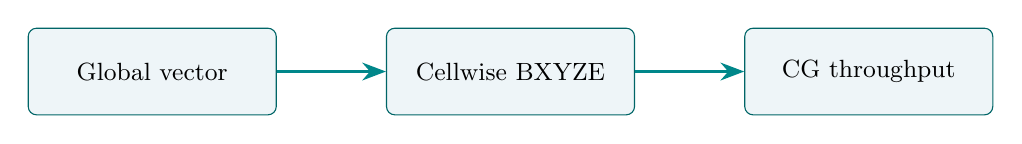
\begin{tikzpicture}[x=1cm,y=1cm]
    \node[flowbox,minimum width=3.15cm] (g) at (0,0) {Global vector};
    \node[flowbox,minimum width=3.15cm] (c) at (4.55,0) {Cellwise BXYZE};
    \node[flowbox,minimum width=3.15cm] (s) at (9.10,0) {CG throughput};
    \draw[flowarrow] (g) -- (c);
    \draw[flowarrow] (c) -- (s);
  \end{tikzpicture}
  \vspace{0.55cm}
\end{frame}

\begin{frame}{The model problem}
  \vspace{0.2cm}
  \begin{columns}[T,onlytextwidth]
    \begin{column}{0.50\textwidth}
      \begin{block}{Poisson problem}
        Find $u=0$ on $\partial\Omega$ such that
        \[
          \int_{\Omega}\nabla v\cdot\nabla u\,\mathrm{d}x
          = \int_{\Omega}v f\,\mathrm{d}x.
        \]
        \vspace{-0.18cm}
        \begin{center}
          {\small\color{muted}Finite-element discretization}\par\vspace{0.03cm}
          {\Large $A u=b$}
        \end{center}
        \vspace{-0.28cm}
      \end{block}
      \vspace{0.10cm}
      {\small Affine tensor-product $Q_p$ hexahedra:
       $\phi_{ijk}=\ell_i(\xi)\ell_j(\eta)\ell_k(\zeta)$,
       with $(p+1)^3$ nodal values per element.\par}
    \end{column}
    \begin{column}{0.46\textwidth}
      \centering
      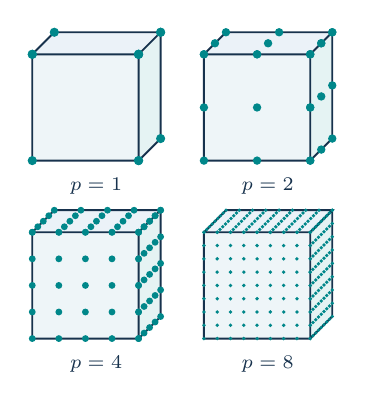
\begin{tikzpicture}
        \ordercube{1}{0}{2.42}
        \ordercube{2}{2.18}{2.42}
        \ordercube{4}{0}{0.16}
        \ordercube{8}{2.18}{0.16}
      \end{tikzpicture}
    \end{column}
  \end{columns}
  \vspace{0.08cm}
  \begin{center}
    {\small\color{ink}$p+1$ Gauss points per direction integrate the
    affine-element stiffness exactly.}
  \end{center}
\end{frame}

\begin{frame}{Classical global matrix-free apply}
  \vspace{0.15cm}
  \begin{center}
    {\Large $\displaystyle y=Ax=\sum_e R_e^{\mathsf T}A_eR_e x$}\par
    \vspace{0.14cm}
    {\small\color{muted}$R_e$ selects the global values belonging to element $e$.}
  \end{center}
  \vspace{0.58cm}
  \begin{center}
  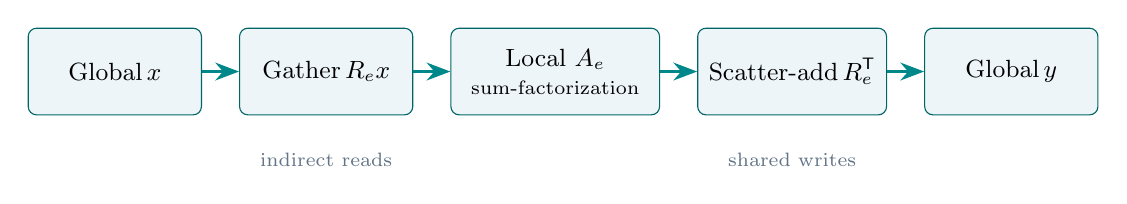
\begin{tikzpicture}[node distance=0.47cm]
    \node[flowbox] (x) {Global\,$x$};
    \node[flowbox,right=of x] (g) {Gather\,$R_e x$};
    \node[flowbox,right=of g,minimum width=2.65cm] (a)
      {Local $A_e$\\[-1pt]\scriptsize sum-factorization};
    \node[flowbox,right=of a] (s) {Scatter-add\,$R_e^{\mathsf T}$};
    \node[flowbox,right=of s] (y) {Global\,$y$};
    \draw[flowarrow] (x) -- (g);
    \draw[flowarrow] (g) -- (a);
    \draw[flowarrow] (a) -- (s);
    \draw[flowarrow] (s) -- (y);
    \node[font=\scriptsize,text=muted,below=0.35cm of g]
      {indirect reads};
    \node[font=\scriptsize,text=muted,below=0.35cm of s]
      {shared writes};
  \end{tikzpicture}
  \end{center}
  \vspace{0.42cm}
  \begin{center}
    \textbf{Focus of this work:} how different memory layouts shape data traffic
    and access patterns around the local operator, especially gather and scatter-add.
  \end{center}
\end{frame}

\begin{frame}{Global gather, local apply, global scatter-add}
  \vspace{-0.10cm}
  \begin{center}
  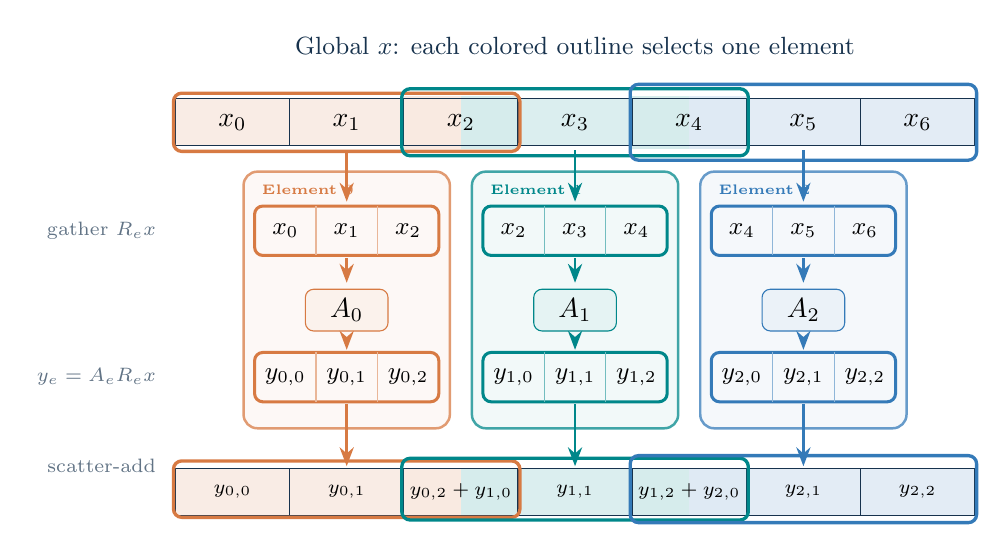
\begin{tikzpicture}[x=1cm,y=1.12cm]
    \node[font=\small,text=ink] at (0,5.52)
      {Global $x$: each colored outline selects one element};
    \foreach \i/\col in
      {0/orange,1/orange,2/pale,3/teal,4/pale,5/blue,6/blue} {
      \pgfmathsetmacro{\xx}{(\i-3)*1.45}
      \node[draw=ink,fill=\col!14,minimum width=1.45cm,minimum height=0.60cm,
            inner sep=0pt] at (\xx,4.65) {$x_{\i}$};
    }
    \fill[orange!16] (-2.175,4.35) rectangle (-1.45,4.95);
    \fill[teal!16] (-1.45,4.35) rectangle (-0.725,4.95);
    \fill[teal!16] (0.725,4.35) rectangle (1.45,4.95);
    \fill[blue!16] (1.45,4.35) rectangle (2.175,4.95);
    \node[draw=ink,minimum width=1.45cm,minimum height=0.60cm,
          inner sep=0pt] at (-1.45,4.65) {$x_2$};
    \node[draw=ink,minimum width=1.45cm,minimum height=0.60cm,
          inner sep=0pt] at (1.45,4.65) {$x_4$};
    \draw[orange,line width=1.2pt,rounded corners=3pt]
      (-5.10,4.32) rectangle (-0.70,4.98);
    \draw[teal,line width=1.2pt,rounded corners=3pt]
      (-2.20,4.27) rectangle (2.20,5.03);
    \draw[blue,line width=1.2pt,rounded corners=3pt]
      (0.70,4.22) rectangle (5.10,5.08);

    \foreach \e/\cx/\col/\first in
      {0/-2.90/orange/0,1/0/teal/2,2/2.90/blue/4} {
      \fill[\col!5,rounded corners=5pt]
        ({\cx-1.31},1.18) rectangle ({\cx+1.31},4.09);
      \draw[draw=\col!75,line width=0.9pt,rounded corners=5pt]
        ({\cx-1.31},1.18) rectangle ({\cx+1.31},4.09);
      \node[font=\tiny\bfseries,text=\col,anchor=west]
        at ({\cx-1.20},3.88) {Element $\e$};
      \draw[-{Stealth[length=2.4mm]},draw=\col,line width=0.9pt]
        (\cx,4.33) -- (\cx,3.75);
      \draw[draw=\col,line width=1.1pt,rounded corners=3pt]
        ({\cx-1.17},3.14) rectangle ({\cx+1.17},3.70);
      \draw[draw=\col!55] ({\cx-0.39},3.14) -- ({\cx-0.39},3.70)
        ({\cx+0.39},3.14) -- ({\cx+0.39},3.70);
      \foreach \j in {0,1,2} {
        \pgfmathtruncatemacro{\gid}{\first+\j}
        \node[font=\small] at ({\cx+(\j-1)*0.78},3.42) {$x_{\gid}$};
        \node[font=\small] at ({\cx+(\j-1)*0.78},1.76) {$y_{\e,\j}$};
      }
      \draw[-{Stealth[length=2.4mm]},draw=\col,line width=0.9pt]
        (\cx,3.11) -- (\cx,2.83);
      \node[draw=\col,fill=\col!10,rounded corners=3pt,
            minimum width=1.05cm,minimum height=0.53cm] at (\cx,2.52)
        {$A_{\e}$};
      \draw[-{Stealth[length=2.4mm]},draw=\col,line width=0.9pt]
        (\cx,2.22) -- (\cx,2.07);
      \draw[draw=\col,line width=1.1pt,rounded corners=3pt]
        ({\cx-1.17},1.48) rectangle ({\cx+1.17},2.04);
      \draw[draw=\col!55] ({\cx-0.39},1.48) -- ({\cx-0.39},2.04)
        ({\cx+0.39},1.48) -- ({\cx+0.39},2.04);
      \draw[-{Stealth[length=2.4mm]},draw=\col,line width=0.9pt]
        (\cx,1.45) -- (\cx,0.75);
    }

    \node[font=\scriptsize,text=muted,anchor=east] at (-5.2,3.42)
      {gather $R_e x$};
    \node[font=\scriptsize,text=muted,anchor=east] at (-5.2,1.76)
      {$y_e=A_eR_ex$};
    \node[font=\scriptsize,text=muted,anchor=east] at (-5.2,0.75)
      {scatter-add};
    \node[draw=ink,fill=orange!14,minimum width=1.45cm,minimum height=0.60cm,
          inner sep=0pt,font=\scriptsize] at (-4.35,0.46) {$y_{0,0}$};
    \node[draw=ink,fill=orange!14,minimum width=1.45cm,minimum height=0.60cm,
          inner sep=0pt,font=\scriptsize] at (-2.90,0.46) {$y_{0,1}$};
    \fill[orange!16] (-2.175,0.19) rectangle (-1.45,0.73);
    \fill[teal!16] (-1.45,0.19) rectangle (-0.725,0.73);
    \node[draw=ink,minimum width=1.45cm,minimum height=0.60cm,
          inner sep=0pt,font=\scriptsize] at (-1.45,0.46) {$y_{0,2}+y_{1,0}$};
    \node[draw=ink,fill=teal!14,minimum width=1.45cm,minimum height=0.60cm,
          inner sep=0pt,font=\scriptsize] at (0,0.46) {$y_{1,1}$};
    \fill[teal!16] (0.725,0.19) rectangle (1.45,0.73);
    \fill[blue!16] (1.45,0.19) rectangle (2.175,0.73);
    \node[draw=ink,minimum width=1.45cm,minimum height=0.60cm,
          inner sep=0pt,font=\scriptsize] at (1.45,0.46) {$y_{1,2}+y_{2,0}$};
    \node[draw=ink,fill=blue!14,minimum width=1.45cm,minimum height=0.60cm,
          inner sep=0pt,font=\scriptsize] at (2.90,0.46) {$y_{2,1}$};
    \node[draw=ink,fill=blue!14,minimum width=1.45cm,minimum height=0.60cm,
          inner sep=0pt,font=\scriptsize] at (4.35,0.46) {$y_{2,2}$};
    \draw[orange,line width=1.2pt,rounded corners=3pt]
      (-5.10,0.17) rectangle (-0.70,0.81);
    \draw[teal,line width=1.2pt,rounded corners=3pt]
      (-2.20,0.14) rectangle (2.20,0.84);
    \draw[blue,line width=1.2pt,rounded corners=3pt]
      (0.70,0.11) rectangle (5.10,0.87);
  \end{tikzpicture}
  \end{center}
  \vspace{-0.18cm}
  {\scriptsize\color{muted}One-dimensional $Q_2$ schematic; the hexahedral
   operator uses $(p+1)^3$ local values per element.}
\end{frame}

\begin{frame}{Bottlenecks of an element-parallel global apply}
  \vspace{0.18cm}
  \begin{columns}[T,onlytextwidth]
    \begin{column}{0.43\textwidth}
      \centering
      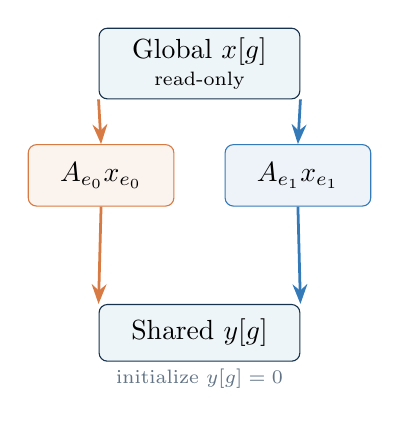
\begin{tikzpicture}[x=1cm,y=1cm]
        \node[draw=ink,fill=pale,rounded corners=3pt,
              minimum width=2.55cm,minimum height=0.72cm,align=center]
              (x) at (2.35,4.30) {Global $x[g]$\\[-2pt]\scriptsize read-only};
        \node[draw=orange,fill=orange!9,rounded corners=3pt,
              minimum width=1.85cm,minimum height=0.78cm]
              (e0) at (1.10,2.88) {$A_{e_0}x_{e_0}$};
        \node[draw=blue,fill=blue!9,rounded corners=3pt,
              minimum width=1.85cm,minimum height=0.78cm]
              (e1) at (3.60,2.88) {$A_{e_1}x_{e_1}$};
        \node[draw=ink,fill=pale,rounded corners=3pt,
              minimum width=2.55cm,minimum height=0.72cm]
              (y) at (2.35,0.88) {Shared $y[g]$};
        \draw[-{Stealth[length=2.5mm]},draw=orange,line width=1pt]
              (x.south west) -- (e0.north);
        \draw[-{Stealth[length=2.5mm]},draw=blue,line width=1pt]
              (x.south east) -- (e1.north);
        \draw[-{Stealth[length=2.5mm]},draw=orange,line width=1pt]
              (e0.south) -- (y.north west);
        \draw[-{Stealth[length=2.5mm]},draw=blue,line width=1pt]
              (e1.south) -- (y.north east);
        \node[font=\scriptsize,text=muted] at (2.35,0.30)
              {initialize $y[g]=0$};
      \end{tikzpicture}
    \end{column}
    \begin{column}{0.55\textwidth}
      \vspace{0.08cm}
      \small
      \begin{itemize}
        \setlength{\itemsep}{0.27cm}
        \item \textbf{Shared writes.} Both elements update the same $y[g]$.
              Parallel scatter-add needs atomics, coloring, or a reduction.
        \item \textbf{Separate output.} In-place $x\leftarrow Ax$ corrupts
              pending reads, and scatter-add would include the old $x$.
              Accumulate into a distinct $y=0$.
        \item \textbf{SIMD across elements.} The baseline processes one element
              at a time. Batching global values needs indexed accesses
              or repacking.
      \end{itemize}
    \end{column}
  \end{columns}
  \vspace{0.12cm}
  {\footnotesize\color{muted}Structured node indices can be implicit;
   shared output writes remain.}
\end{frame}

\begin{frame}{Cellwise apply: element-local copies}
  \vspace{-0.10cm}
  \begin{center}
  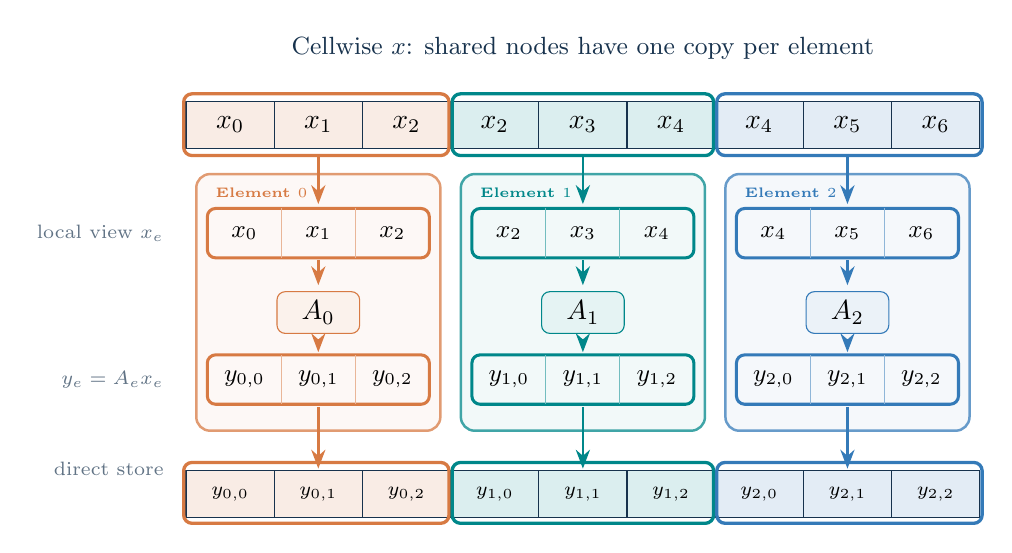
\begin{tikzpicture}[x=1cm,y=1.12cm]
    \node[font=\small,text=ink] at (0,5.52)
      {Cellwise $x$: shared nodes have one copy per element};
    \foreach \i/\gid/\col in
      {0/0/orange,1/1/orange,2/2/orange,
       3/2/teal,4/3/teal,5/4/teal,
       6/4/blue,7/5/blue,8/6/blue} {
      \pgfmathsetmacro{\xx}{(\i-4)*1.12}
      \node[draw=ink,fill=\col!14,minimum width=1.12cm,
            minimum height=0.60cm,inner sep=0pt] at (\xx,4.65) {$x_{\gid}$};
    }
    \draw[orange,line width=1.2pt,rounded corners=3pt]
      (-5.07,4.30) rectangle (-1.70,5.00);
    \draw[teal,line width=1.2pt,rounded corners=3pt]
      (-1.66,4.30) rectangle (1.66,5.00);
    \draw[blue,line width=1.2pt,rounded corners=3pt]
      (1.70,4.30) rectangle (5.07,5.00);

    \foreach \e/\cx/\col/\first in
      {0/-3.36/orange/0,1/0/teal/2,2/3.36/blue/4} {
      \fill[\col!5,rounded corners=5pt]
        ({\cx-1.55},1.18) rectangle ({\cx+1.55},4.09);
      \draw[draw=\col!75,line width=0.9pt,rounded corners=5pt]
        ({\cx-1.55},1.18) rectangle ({\cx+1.55},4.09);
      \node[font=\tiny\bfseries,text=\col,anchor=west]
        at ({\cx-1.43},3.88) {Element $\e$};
      \draw[-{Stealth[length=2.4mm]},draw=\col,line width=0.9pt]
        (\cx,4.30) -- (\cx,3.75);
      \draw[draw=\col,line width=1.1pt,rounded corners=3pt]
        ({\cx-1.41},3.14) rectangle ({\cx+1.41},3.70);
      \draw[draw=\col!55] ({\cx-0.47},3.14) -- ({\cx-0.47},3.70)
        ({\cx+0.47},3.14) -- ({\cx+0.47},3.70);
      \foreach \j in {0,1,2} {
        \pgfmathtruncatemacro{\gid}{\first+\j}
        \node[font=\small] at ({\cx+(\j-1)*0.94},3.42) {$x_{\gid}$};
        \node[font=\small] at ({\cx+(\j-1)*0.94},1.76) {$y_{\e,\j}$};
      }
      \draw[-{Stealth[length=2.4mm]},draw=\col,line width=0.9pt]
        (\cx,3.11) -- (\cx,2.83);
      \node[draw=\col,fill=\col!10,rounded corners=3pt,
            minimum width=1.05cm,minimum height=0.53cm] at (\cx,2.52)
        {$A_{\e}$};
      \draw[-{Stealth[length=2.4mm]},draw=\col,line width=0.9pt]
        (\cx,2.22) -- (\cx,2.07);
      \draw[draw=\col,line width=1.1pt,rounded corners=3pt]
        ({\cx-1.41},1.48) rectangle ({\cx+1.41},2.04);
      \draw[draw=\col!55] ({\cx-0.47},1.48) -- ({\cx-0.47},2.04)
        ({\cx+0.47},1.48) -- ({\cx+0.47},2.04);
      \draw[-{Stealth[length=2.4mm]},draw=\col,line width=0.9pt]
        (\cx,1.45) -- (\cx,0.75);
    }

    \node[font=\scriptsize,text=muted,anchor=east] at (-5.2,3.42)
      {local view $x_e$};
    \node[font=\scriptsize,text=muted,anchor=east] at (-5.2,1.76)
      {$y_e=A_ex_e$};
    \node[font=\scriptsize,text=muted,anchor=east] at (-5.2,0.75)
      {direct store};
    \foreach \i/\e/\j/\col in
      {0/0/0/orange,1/0/1/orange,2/0/2/orange,
       3/1/0/teal,4/1/1/teal,5/1/2/teal,
       6/2/0/blue,7/2/1/blue,8/2/2/blue} {
      \pgfmathsetmacro{\xx}{(\i-4)*1.12}
      \node[draw=ink,fill=\col!14,minimum width=1.12cm,
            minimum height=0.60cm,inner sep=0pt,font=\scriptsize]
            at (\xx,0.46) {$y_{\e,\j}$};
    }
    \draw[orange,line width=1.2pt,rounded corners=3pt]
      (-5.07,0.13) rectangle (-1.70,0.82);
    \draw[teal,line width=1.2pt,rounded corners=3pt]
      (-1.66,0.13) rectangle (1.66,0.82);
    \draw[blue,line width=1.2pt,rounded corners=3pt]
      (1.70,0.13) rectangle (5.07,0.82);
  \end{tikzpicture}
  \end{center}
  \vspace{-0.18cm}
  {\scriptsize\color{muted}Logical element view; BXYZE interleaves lanes.
   DSS later sums shared outputs.}
\end{frame}

\begin{frame}{BXYZE: explicit offsets and padded blocks}
  \vspace{-0.08cm}
  \begin{center}
    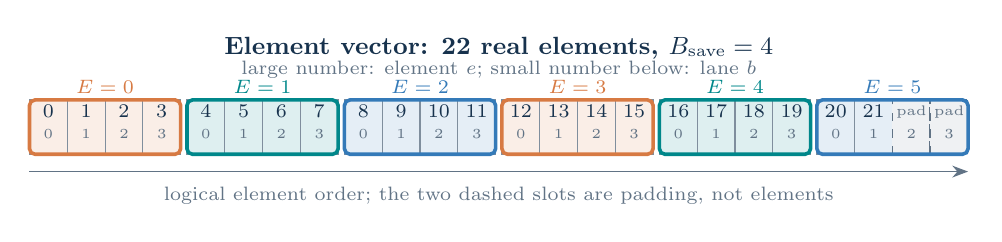
\begin{tikzpicture}[x=1cm,y=1cm]
      \node[font=\small\bfseries,text=ink] at (6.06,2.06)
        {Element vector: 22 real elements, $B_{\mathrm{save}}=4$};
      \node[font=\scriptsize,text=muted] at (6.06,1.78)
        {large number: element $e$; small number below: lane $b$};
      \foreach \E/\col in
        {0/orange,1/teal,2/blue,3/orange,4/teal,5/blue} {
        \pgfmathsetmacro{\xbase}{0.10+2.00*\E}
        \foreach \b in {0,1,2,3} {
          \pgfmathtruncatemacro{\eid}{4*\E+\b}
          \ifnum\eid<22
            \fill[\col!13] ({\xbase+0.48*\b},0.71)
              rectangle ({\xbase+0.48*(\b+1)},1.40);
            \draw[ink!55,line width=0.4pt]
              ({\xbase+0.48*\b},0.71)
              rectangle ({\xbase+0.48*(\b+1)},1.40);
            \node[font=\scriptsize,text=ink]
              at ({\xbase+0.48*(\b+0.5)},1.25) {\eid};
          \else
            \fill[muted!10] ({\xbase+0.48*\b},0.71)
              rectangle ({\xbase+0.48*(\b+1)},1.40);
            \draw[muted,dashed,line width=0.7pt]
              ({\xbase+0.48*\b},0.71)
              rectangle ({\xbase+0.48*(\b+1)},1.40);
            \node[font=\tiny,text=muted]
              at ({\xbase+0.48*(\b+0.5)},1.25) {pad};
          \fi
          \node[font=\tiny,text=muted]
            at ({\xbase+0.48*(\b+0.5)},0.97) {\b};
        }
        \draw[\col,line width=1.3pt,rounded corners=2pt]
          (\xbase,0.71) rectangle ({\xbase+1.92},1.40);
        \node[font=\scriptsize\bfseries,text=\col]
          at ({\xbase+0.96},1.57) {$E=\E$};
      }
      \draw[-{Stealth[length=2mm]},draw=muted,line width=0.6pt]
        (0.10,0.49) -- (12.02,0.49);
      \node[font=\scriptsize,text=muted] at (6.06,0.18)
        {logical element order; the two dashed slots are padding, not elements};
    \end{tikzpicture}
  \end{center}
  \vspace{-0.21cm}
  \begin{columns}[T,onlytextwidth]
    \begin{column}{0.46\textwidth}
      {\scriptsize\color{muted}Logical index order, slowest to fastest\par}
      \vspace{0.12cm}
      {\Large\color{teal}$u[E][z][y][x][b]$\par}
      \vspace{0.14cm}
      {\small
        $E$: storage block; $b$: lane.\par
        \vspace{0.11cm}
        $e=E B_{\mathrm{save}}+b$.\par
        \vspace{0.11cm}
        $x,y,z$: local nodal indices, $N=p+1$.
      }
    \end{column}
    \begin{column}{0.52\textwidth}
      {\small\bfseries Explicit scalar offset\par}
      \vspace{0.12cm}
      {\small
        $v=x+N(y+Nz)$ (local node).\par
        \vspace{0.15cm}
        $\mathrm{off}(E,v,b)=(E N^3+v)B_{\mathrm{save}}+b$.\par
        \vspace{0.15cm}
        Fixed $(E,v)$: $\mathrm{off}(b+1)=\mathrm{off}(b)+1$.\par
        \vspace{0.12cm}
        Lanes of one block are contiguous for SIMD.
      }
    \end{column}
  \end{columns}
  \vspace{0.12cm}
  \begin{block}{What padding means}
    \footnotesize Each block stores $N^3 B_{\mathrm{save}}$ values.
    In $E=5$, lanes $b=2,3$ have no element and are zero-filled by conversion.
    The offset formula remains valid. The current affine apply requires full blocks.
  \end{block}
\end{frame}

\begin{frame}{BXYZE: $b$ is the fastest index (1/4)}
  \bxyzelanestep{0}
\end{frame}

\begin{frame}{BXYZE: $b$ is the fastest index (2/4)}
  \bxyzelanestep{1}
\end{frame}

\begin{frame}{BXYZE: $b$ is the fastest index (3/4)}
  \bxyzelanestep{2}
\end{frame}

\begin{frame}{BXYZE: $b$ is the fastest index (4/4)}
  \bxyzelanestep{3}
\end{frame}

\begin{frame}{Cellwise: benefits and costs}
  \vspace{-0.20cm}
  \begin{columns}[T,onlytextwidth]
    \begin{column}{0.48\textwidth}
      \begin{block}{Benefits}
        \small
        \begin{itemize}
          \setlength{\itemsep}{0.08cm}
          \item \textbf{SIMD:} lanes for the same local node are contiguous.
          \item \textbf{No write conflicts:} the local apply needs no
                atomics or coloring.
        \end{itemize}
      \end{block}
    \end{column}
    \begin{column}{0.48\textwidth}
      {\setbeamercolor{block title}{fg=white,bg=orange}
       \setbeamercolor{block body}{fg=ink,bg=orange!8}
       \begin{block}{Costs}
         \small
         \begin{itemize}
           \setlength{\itemsep}{0.08cm}
           \item Shared-node contributions still need summation (DSS).
           \item Duplicated nodal values increase memory per cellwise vector.
         \end{itemize}
       \end{block}}
    \end{column}
  \end{columns}

  \vspace{0.05cm}
  {\large\bfseries Extra nodal storage for $64^3$ elements\par}
  \vspace{0.06cm}
  {\small $N_{\mathrm{global}}=(64p+1)^3$,\quad
          $N_{\mathrm{cell}}=64^3(p+1)^3$.\par}
  \vspace{0.02cm}
  \begin{center}
    {\small
    \begin{tabular}{c r r r r}
      \hline
      $p$ & Global nodes & Cellwise entries & Extra copies & Extra FP64 memory \\
      \hline
      2 & $2\,146\,689$ & $7\,077\,888$ & $4\,931\,199$ & $37.6$ MiB \\
      4 & $16\,974\,593$ & $32\,768\,000$ & $15\,793\,407$ & $120.5$ MiB \\
      8 & $135\,005\,697$ & $191\,102\,976$ & $56\,097\,279$ & $428.0$ MiB \\
      \hline
    \end{tabular}}
  \end{center}
  \vspace{-0.16cm}
  {\small\color{orange}\textbf{At $128^3$ elements, $p=8$:}
   $451\,933\,183$ extra entries $\Rightarrow$ \textbf{3.37 GiB} per FP64 vector.\par}
  \vspace{0.05cm}
  {\scriptsize\color{muted}Assumes full blocks; geometry and workspace excluded.\par}
\end{frame}

\begin{frame}{Structured DSS: each element meets its neighbor}
  \vspace{-0.07cm}
  \begin{center}
    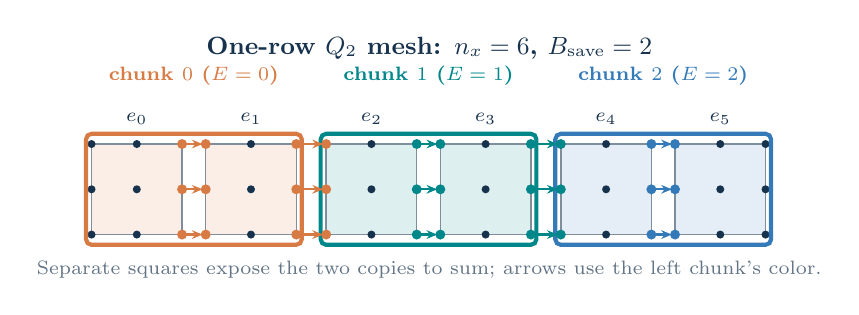
\begin{tikzpicture}[x=1cm,y=1cm]
      \node[font=\small\bfseries,text=ink] at (6.07,3.02)
        {One-row $Q_2$ mesh: $n_x=6$, $B_{\mathrm{save}}=2$};
      \foreach \E/\col in {0/orange,1/teal,2/blue} {
        \pgfmathsetmacro{\xbase}{1.78+2.98*\E}
        \foreach \b in {0,1} {
          \pgfmathtruncatemacro{\eid}{2*\E+\b}
          \fill[\col!13] ({\xbase+1.45*\b},0.65)
            rectangle ({\xbase+1.45*\b+1.15},1.80);
          \draw[ink!55,line width=0.5pt]
            ({\xbase+1.45*\b},0.65)
            rectangle ({\xbase+1.45*\b+1.15},1.80);
          \foreach \ix in {0,1,2} {
            \foreach \iy in {0,1,2} {
              \fill[ink]
                ({\xbase+1.45*\b+0.575*\ix},{0.65+0.575*\iy})
                circle (1.45pt);
            }
          }
          \node[font=\scriptsize,text=ink]
            at ({\xbase+1.45*\b+0.575},2.12) {$e_{\eid}$};
        }
        \draw[\col,line width=1.5pt,rounded corners=2pt]
          ({\xbase-0.07},0.52) rectangle ({\xbase+2.67},1.93);
        \node[font=\scriptsize\bfseries,text=\col]
          at ({\xbase+1.30},2.67) {chunk $\E$ ($E=\E$)};
      }
      \foreach \i/\col in {0/orange,1/orange,2/teal,3/teal,4/blue} {
        \pgfmathtruncatemacro{\lgroup}{floor(\i/2)}
        \pgfmathtruncatemacro{\llane}{mod(\i,2)}
        \pgfmathtruncatemacro{\rgroup}{floor((\i+1)/2)}
        \pgfmathtruncatemacro{\rlane}{mod(\i+1,2)}
        \pgfmathsetmacro{\xleft}{1.78+2.98*\lgroup+1.45*\llane+1.15}
        \pgfmathsetmacro{\xright}{1.78+2.98*\rgroup+1.45*\rlane}
        \foreach \iy in {0,1,2} {
          \pgfmathsetmacro{\ynode}{0.65+0.575*\iy}
          \draw[-{Stealth[length=1.35mm,width=1.1mm]},draw=\col,line width=0.85pt]
            ({\xleft+0.04},\ynode) -- ({\xright-0.04},\ynode);
          \fill[\col] (\xleft,\ynode) circle (1.8pt);
          \fill[\col] (\xright,\ynode) circle (1.8pt);
        }
      }
      \node[font=\scriptsize,text=muted] at (6.07,0.21)
        {Separate squares expose the two copies to sum; arrows use the left chunk's color.};
    \end{tikzpicture}
  \end{center}
  \vspace{-0.17cm}
  \begin{columns}[T,onlytextwidth]
    \begin{column}{0.46\textwidth}
      {\small\bfseries In 3D: three ordered passes\par}
      \vspace{0.08cm}
      {\Large\color{teal}$z\ \longrightarrow\ y\ \longrightarrow\ x$\par}
      \vspace{0.09cm}
      {\small At each interface, sum matching face-node copies and write
       the sum to both elements.\par}
    \end{column}
    \begin{column}{0.51\textwidth}
      {\small\bfseries Numbering gives the neighbor directly\par}
      \vspace{0.08cm}
      {\small
        $e=e_x+n_x(e_y+n_y e_z)$.\par
        \vspace{0.09cm}
        Given $e$, add $1$ in $x$, $n_x$ in $y$, or $n_xn_y$ in $z$
        to find the next element. No connectivity lookup.\par
      }
    \end{column}
  \end{columns}
  \vspace{0.16cm}
  {\scriptsize\color{muted}The $z\to y\to x$ cascade also assembles edge
   and corner nodes; an OpenMP barrier separates the passes.\par}
\end{frame}

\begin{frame}{Operator throughput: $16^3$ elements}
  \noindent\makebox[\linewidth][c]{%
    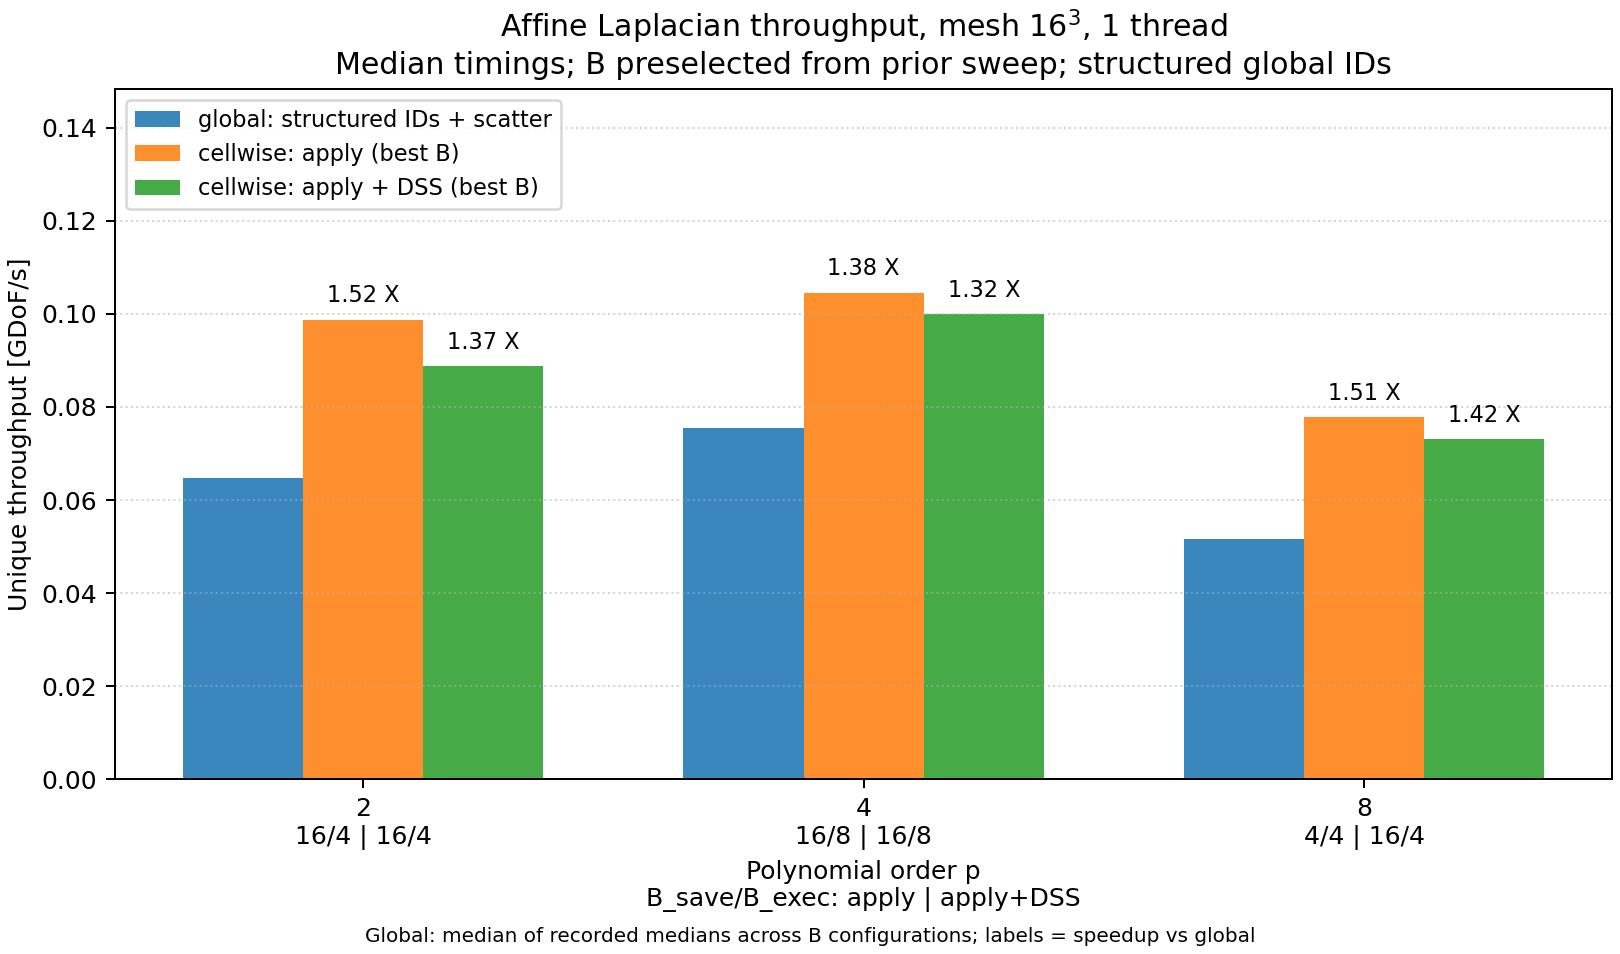
\includegraphics[width=0.49\paperwidth]{dss_bxyze_affine_laplacian_global_gdof_s_unique_n16_t1_structured_boundary_atomic_median.png}%
    \hspace{0.01\paperwidth}%
    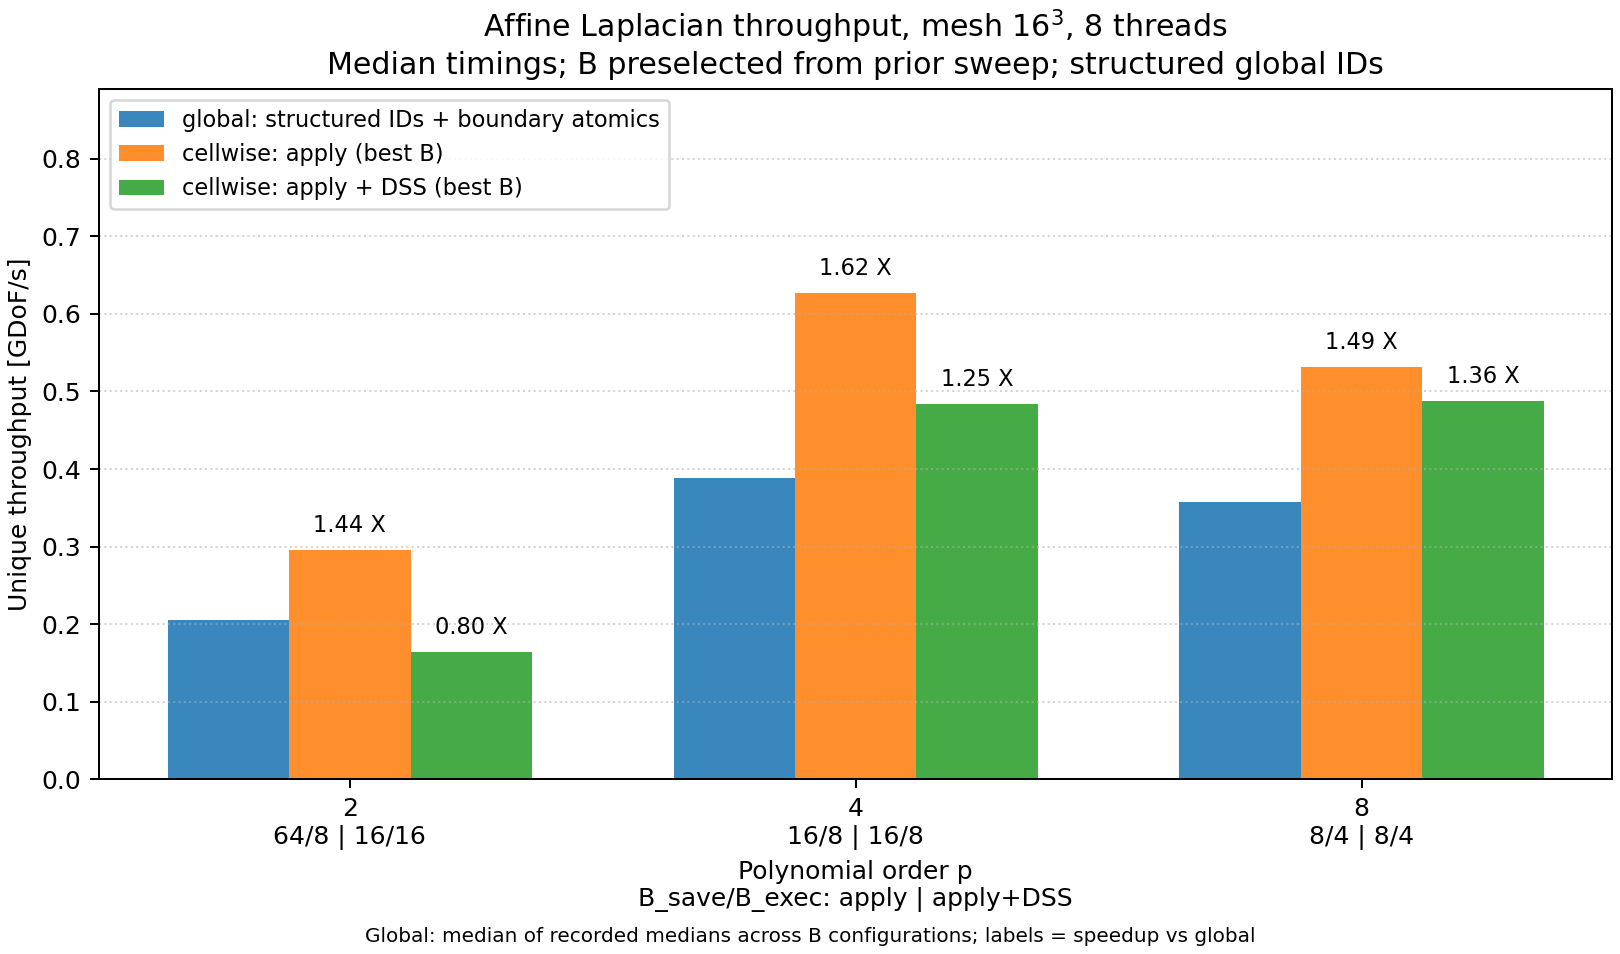
\includegraphics[width=0.49\paperwidth]{dss_bxyze_affine_laplacian_global_gdof_s_unique_n16_t8_structured_boundary_atomic_median.png}%
  }\par
  \vspace{0.22cm}
  {\centering\small\color{muted}Throughput in unique global DoFs/s; speedups are relative to the global apply.\par}
\end{frame}

\begin{frame}{Operator throughput: $64^3$ elements}
  \noindent\makebox[\linewidth][c]{%
    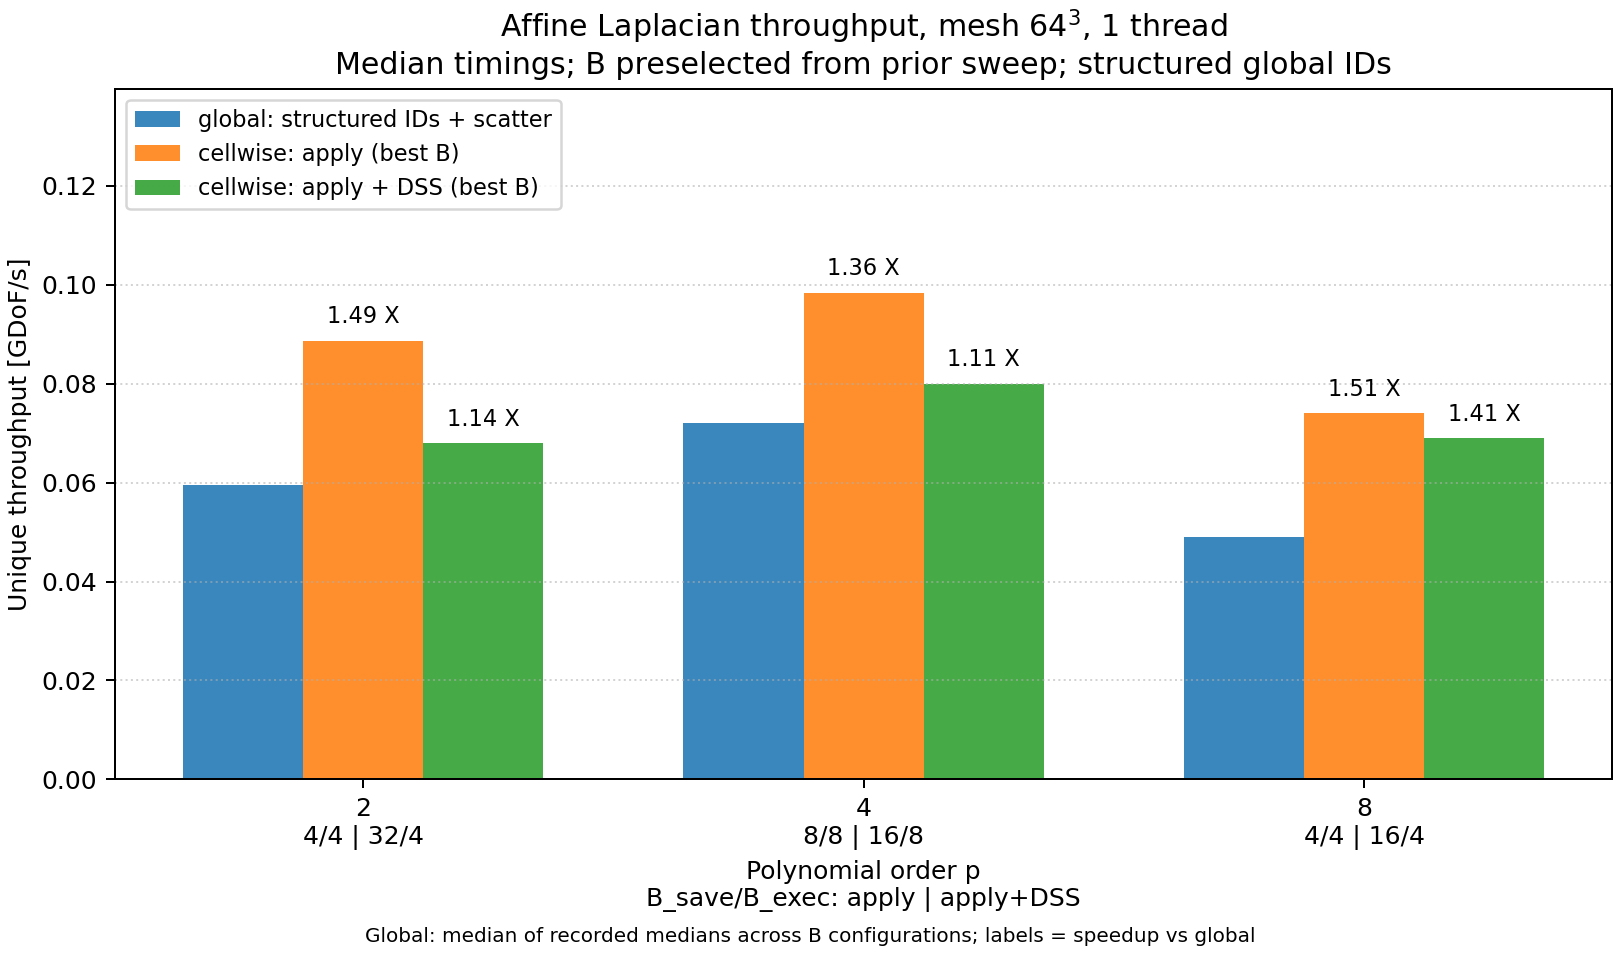
\includegraphics[width=0.49\paperwidth]{dss_bxyze_affine_laplacian_global_gdof_s_unique_n64_t1_structured_boundary_atomic_median.png}%
    \hspace{0.01\paperwidth}%
    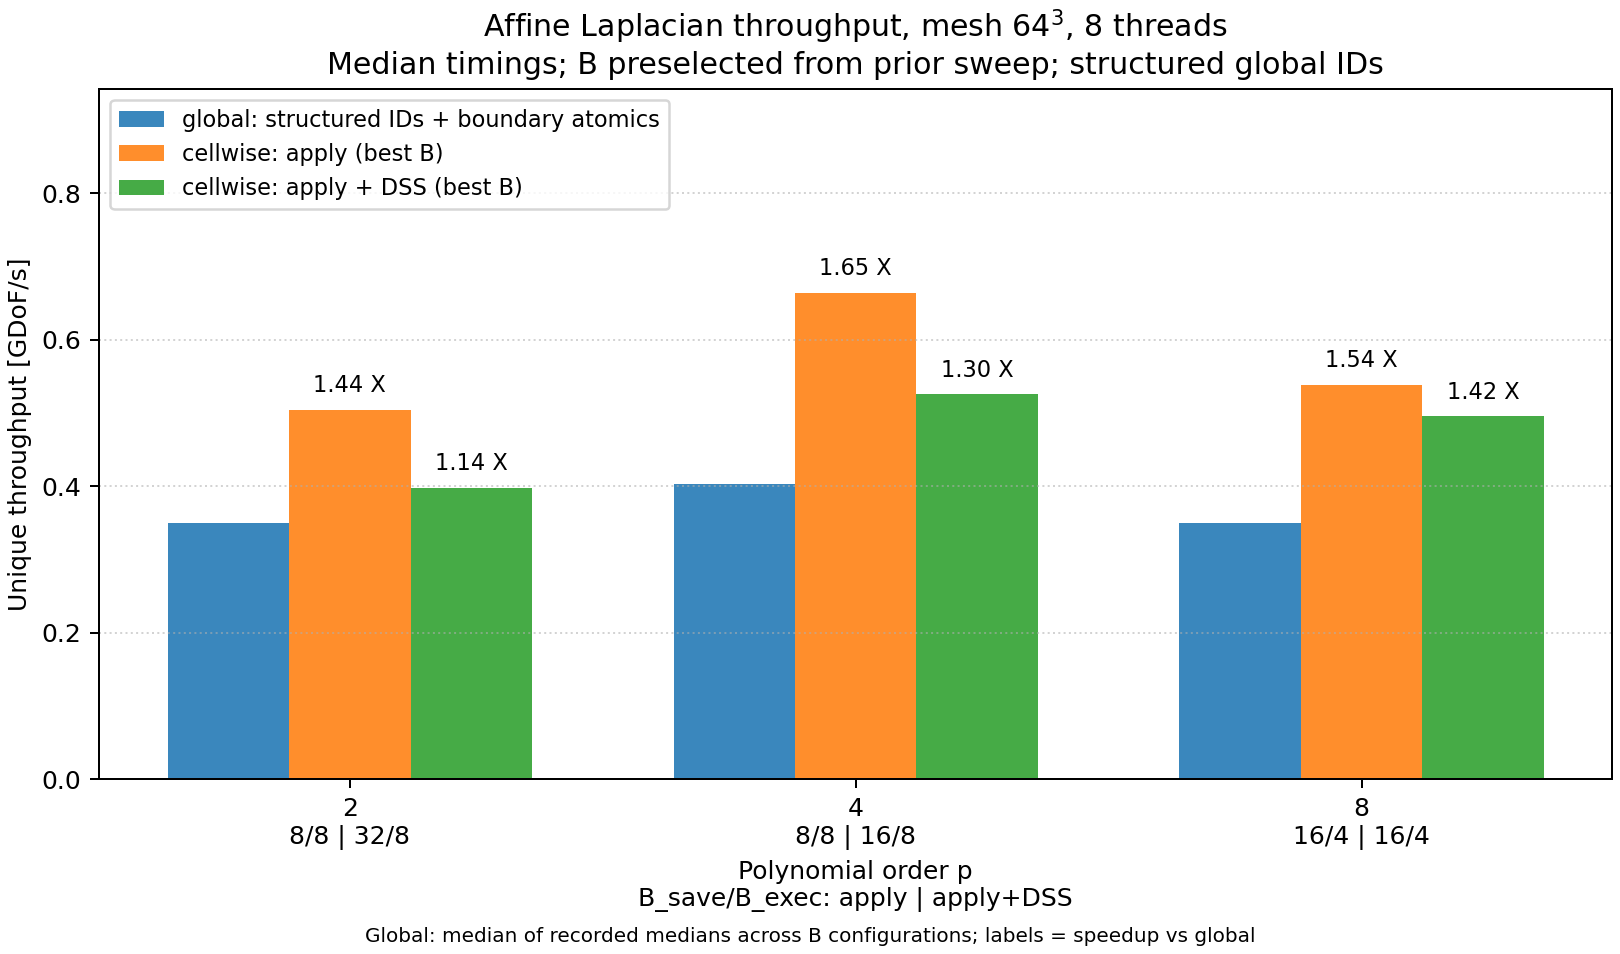
\includegraphics[width=0.49\paperwidth]{dss_bxyze_affine_laplacian_global_gdof_s_unique_n64_t8_structured_boundary_atomic_median.png}%
  }\par
  \vspace{0.22cm}
  {\centering\small\color{muted}Throughput in unique global DoFs/s; speedups are relative to the global apply.\par}
\end{frame}

\begin{frame}{CG throughput: 1 thread}
  \noindent\makebox[\linewidth][c]{%
    \begin{minipage}[t]{0.49\paperwidth}\vspace{0pt}%
      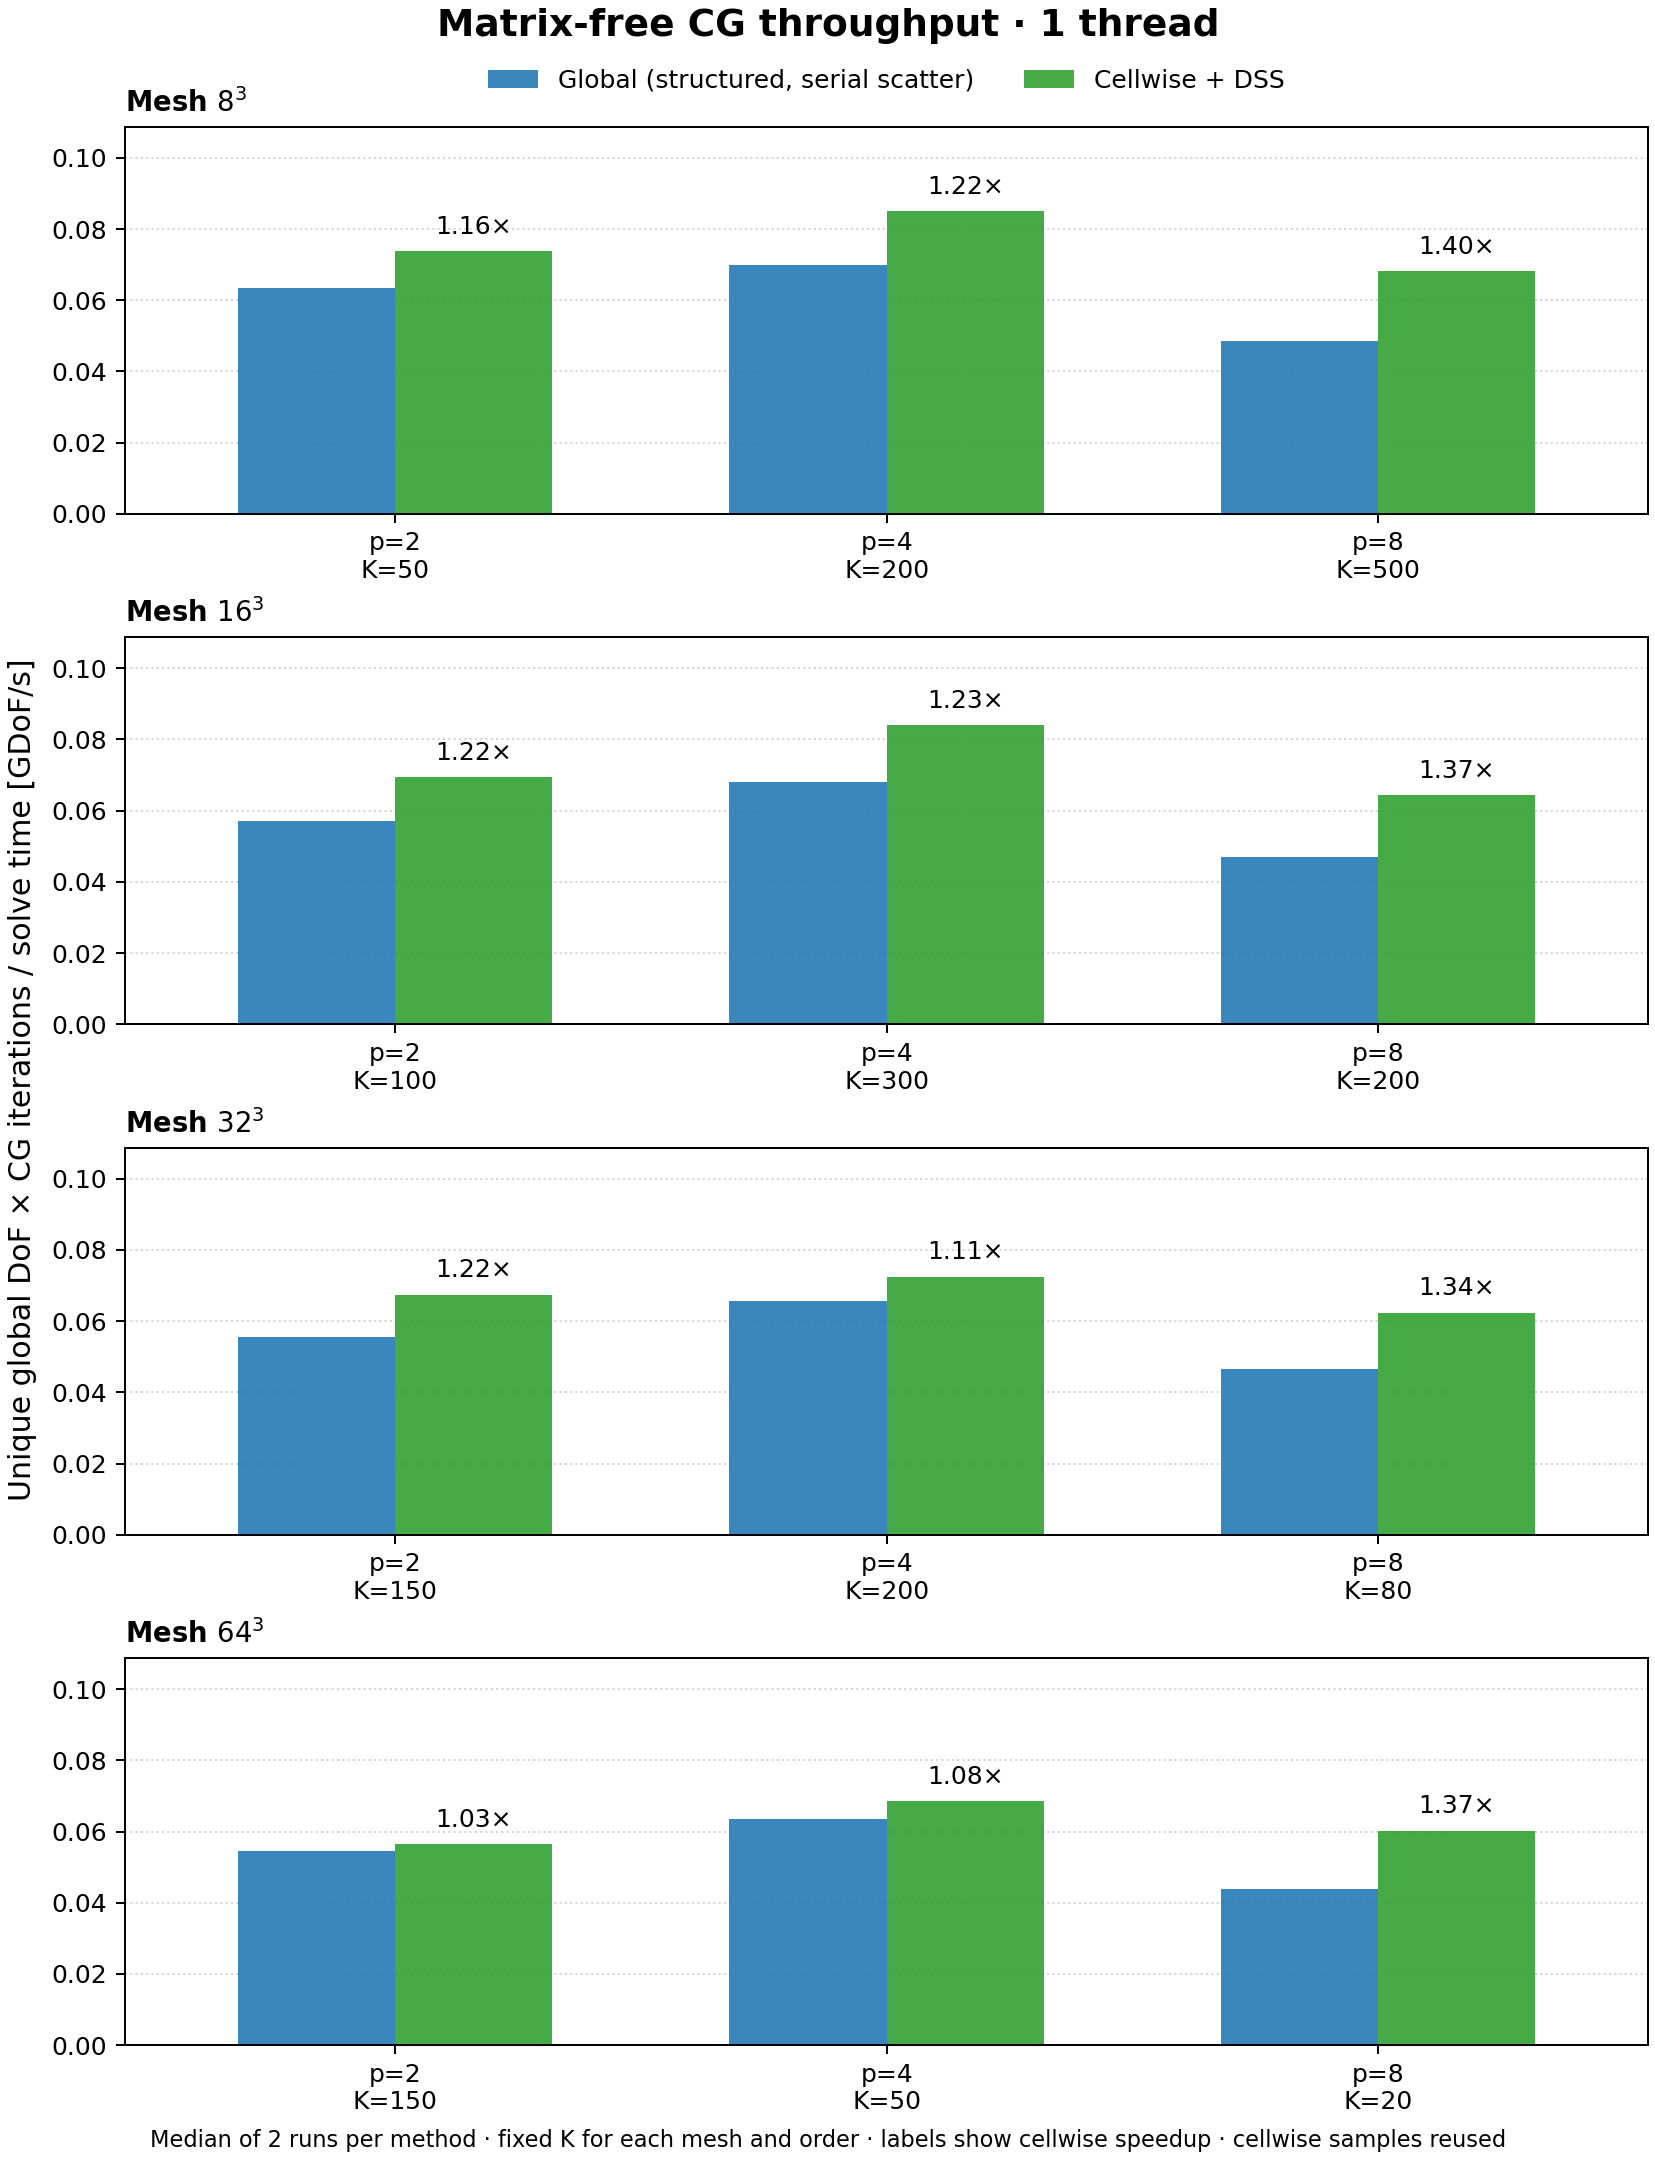
\includegraphics[width=\linewidth,trim=18bp 432bp 0 18bp,clip]{dss_bxyze_cg_fixed_budget_structured_boundary_released_throughput_t1.png}%
    \end{minipage}%
    \hspace{0.01\paperwidth}%
    \begin{minipage}[t]{0.49\paperwidth}\vspace{0pt}%
      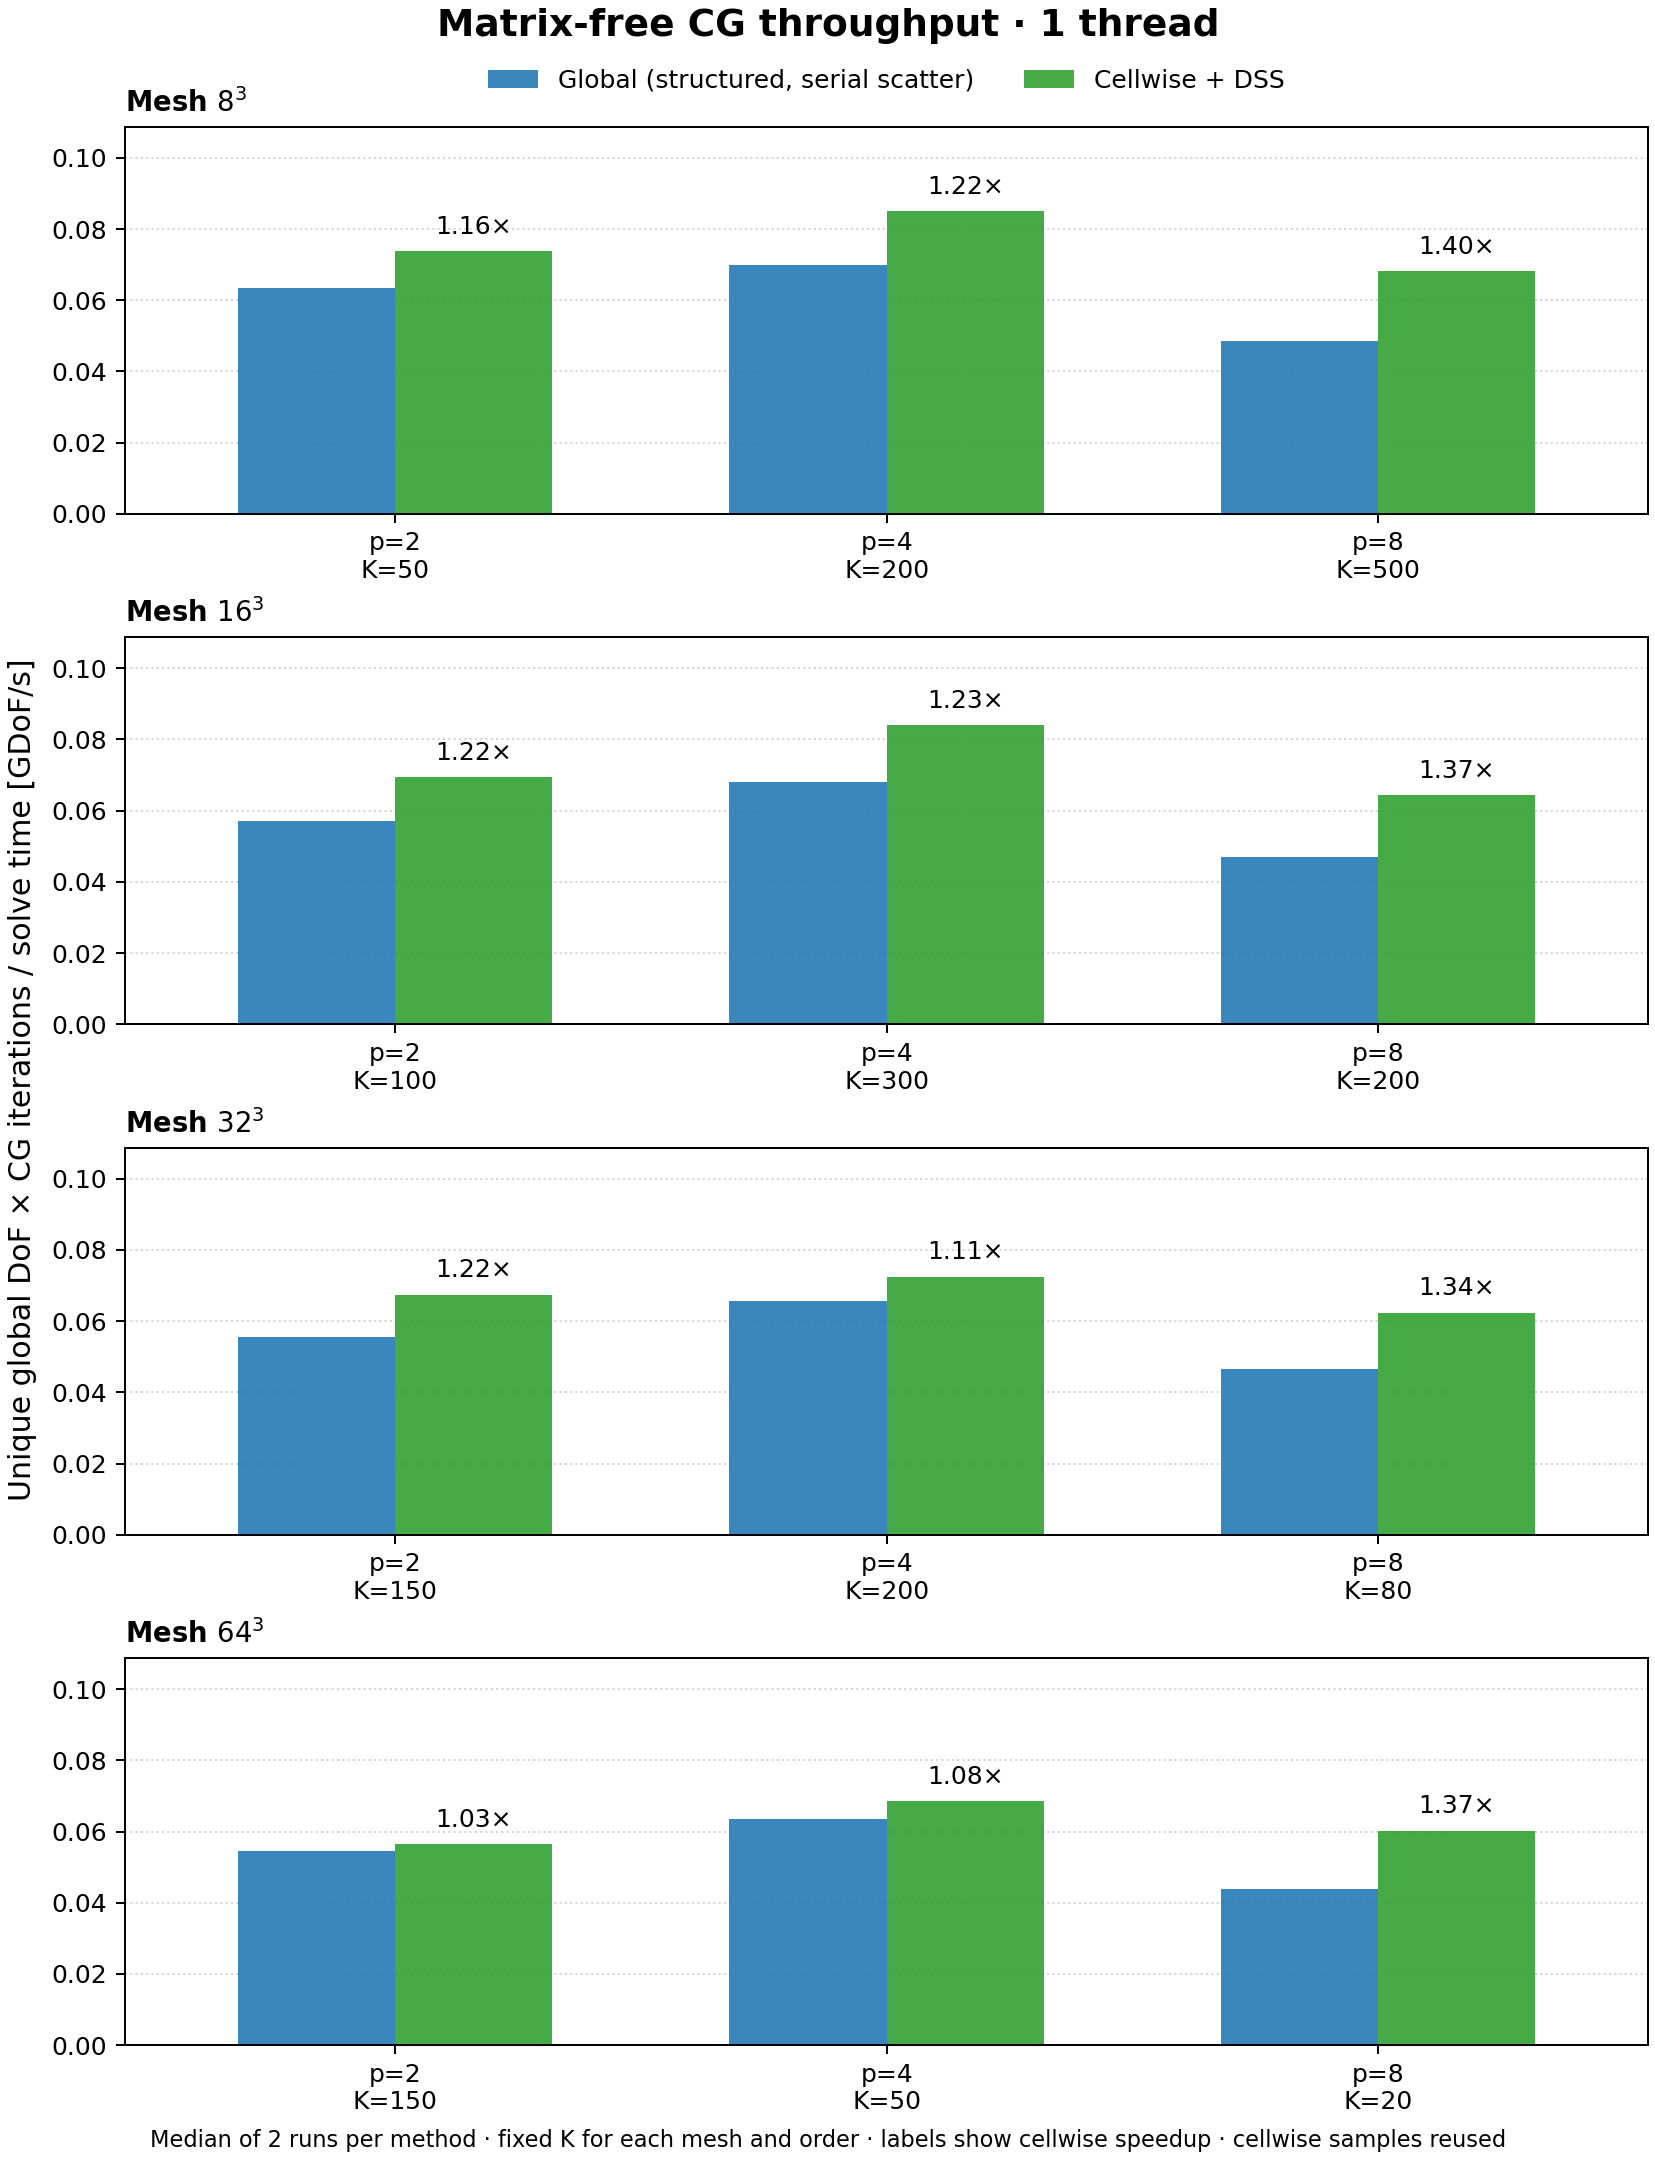
\includegraphics[width=\linewidth,trim=18bp 0 0 432bp,clip]{dss_bxyze_cg_fixed_budget_structured_boundary_released_throughput_t1.png}%
    \end{minipage}%
  }\par
  \vspace{0.13cm}
  {\centering\small\color{muted}Throughput $=\text{unique global DoFs}\times K/\text{solve time}$;
   $K$ is fixed per case.\par}
\end{frame}

\begin{frame}{CG throughput: 8 threads}
  \noindent\makebox[\linewidth][c]{%
    \begin{minipage}[t]{0.49\paperwidth}\vspace{0pt}%
      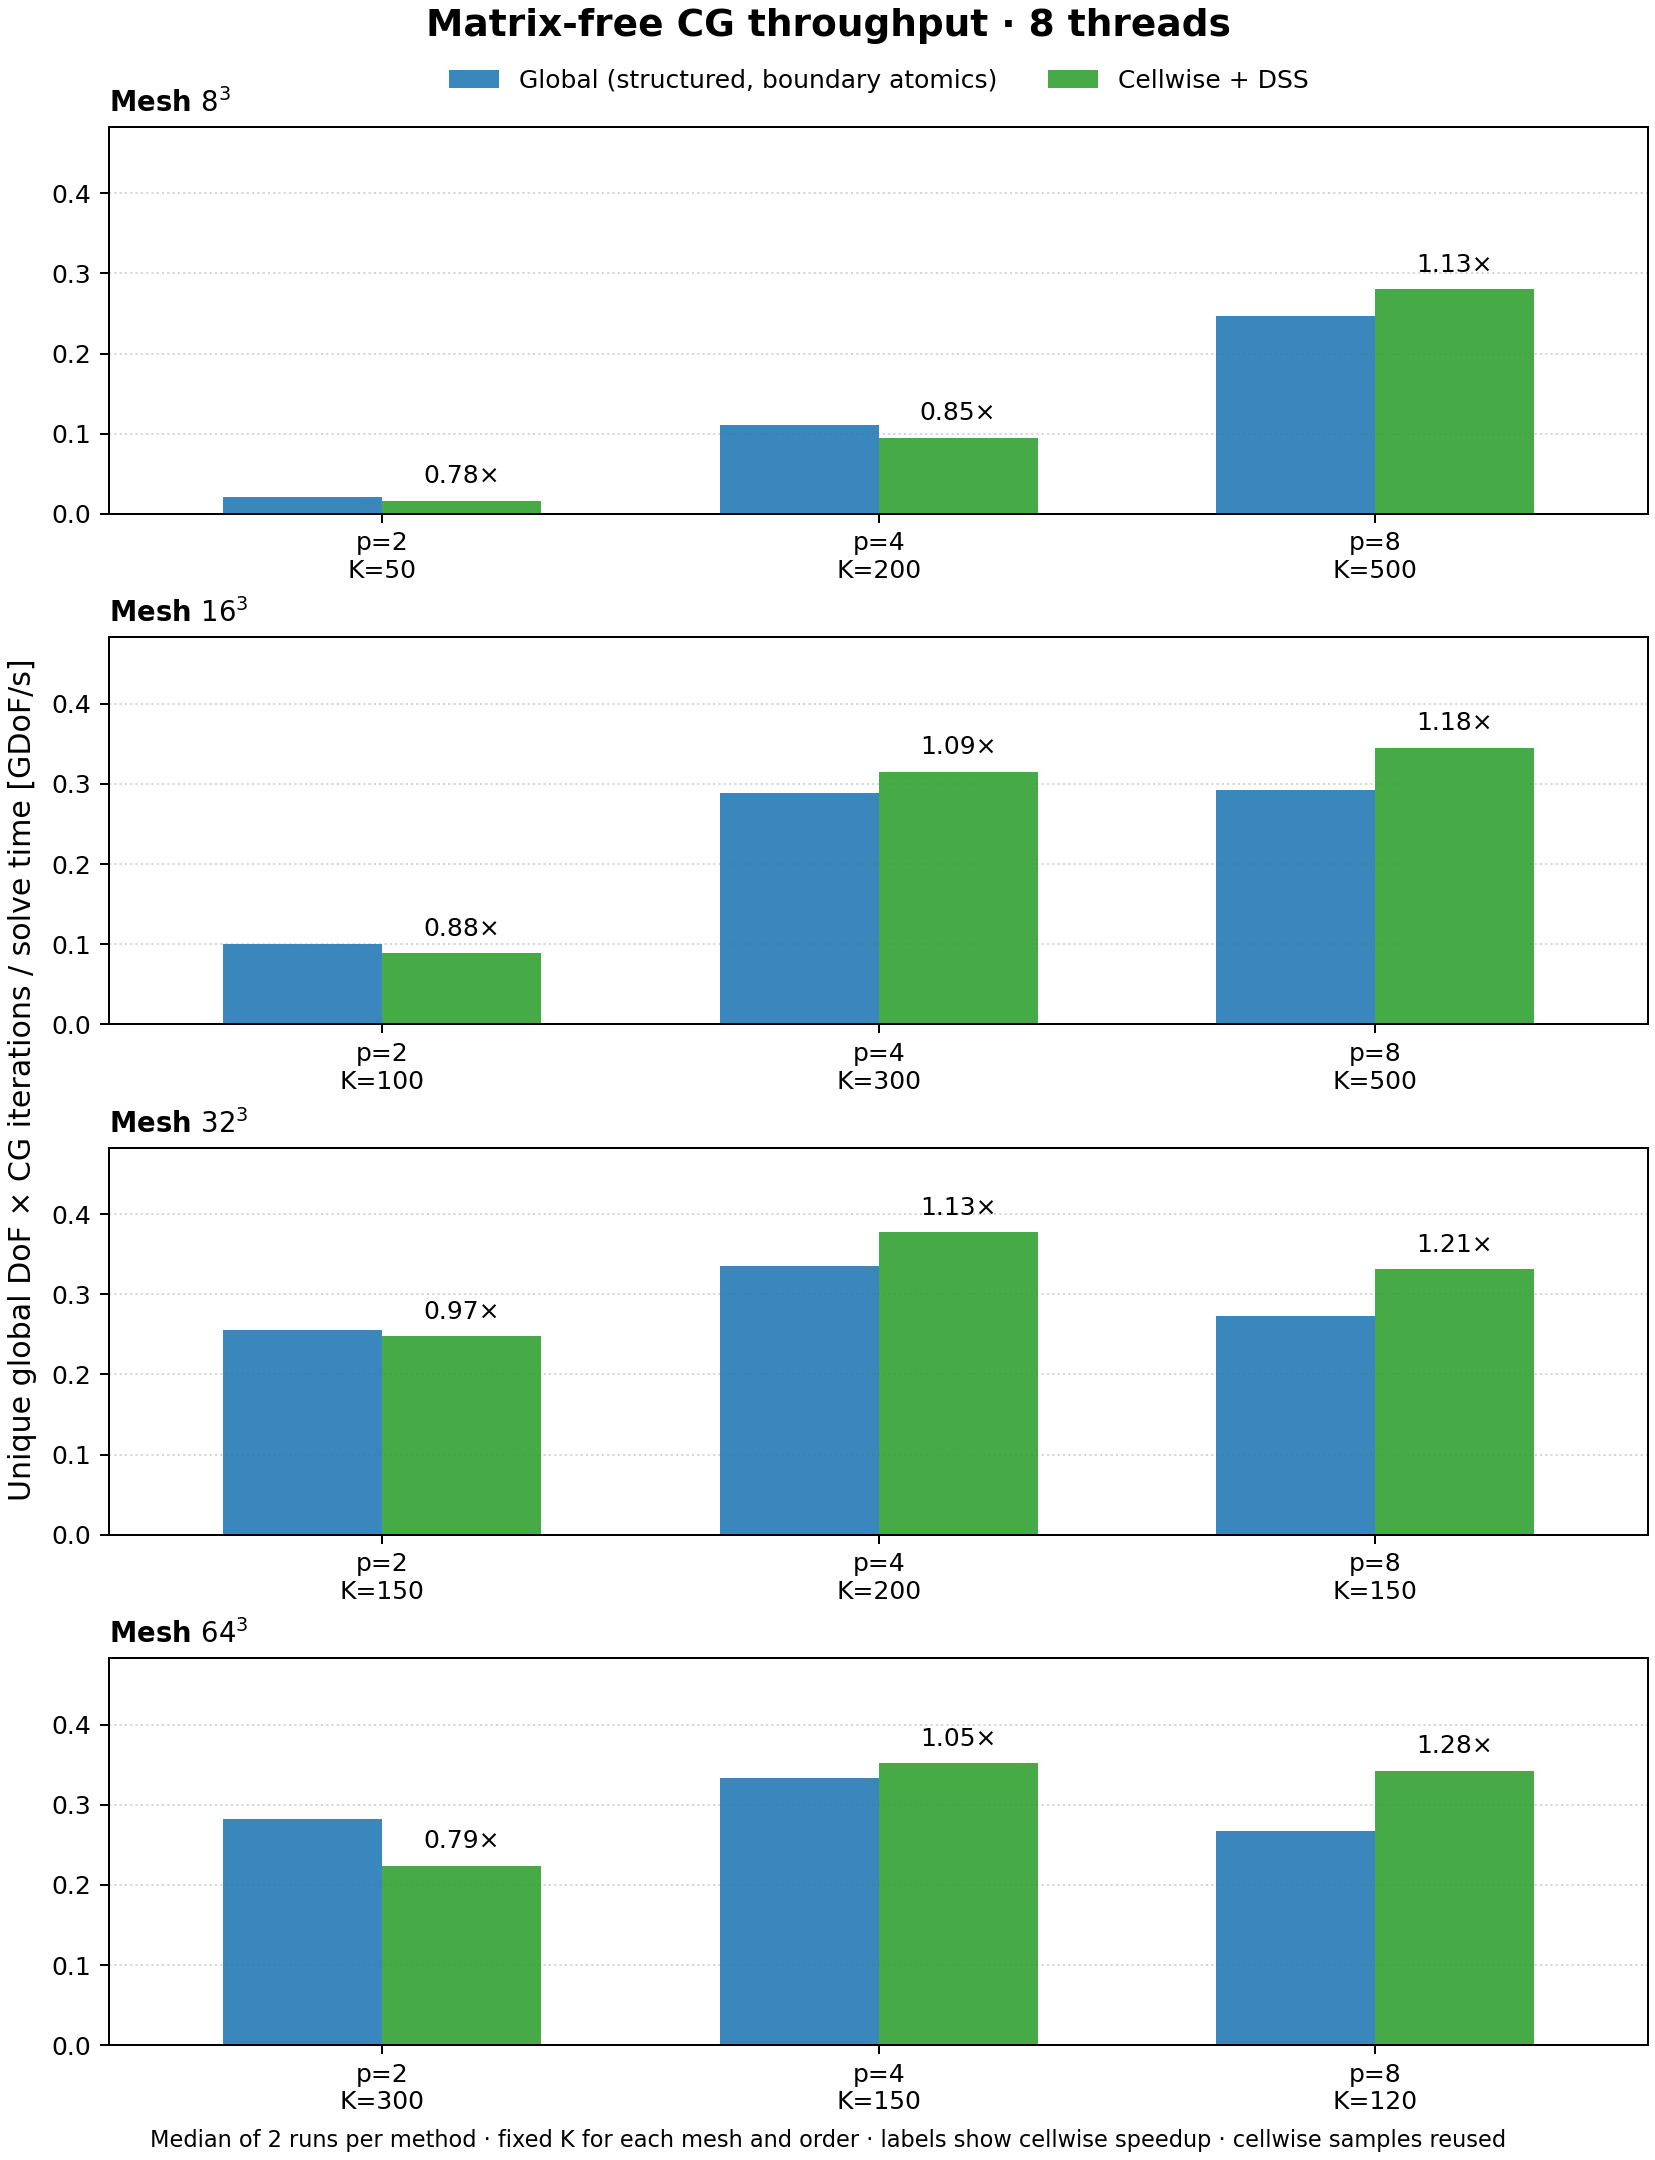
\includegraphics[width=\linewidth,trim=18bp 432bp 0 18bp,clip]{dss_bxyze_cg_fixed_budget_structured_boundary_released_throughput_t8.png}%
    \end{minipage}%
    \hspace{0.01\paperwidth}%
    \begin{minipage}[t]{0.49\paperwidth}\vspace{0pt}%
      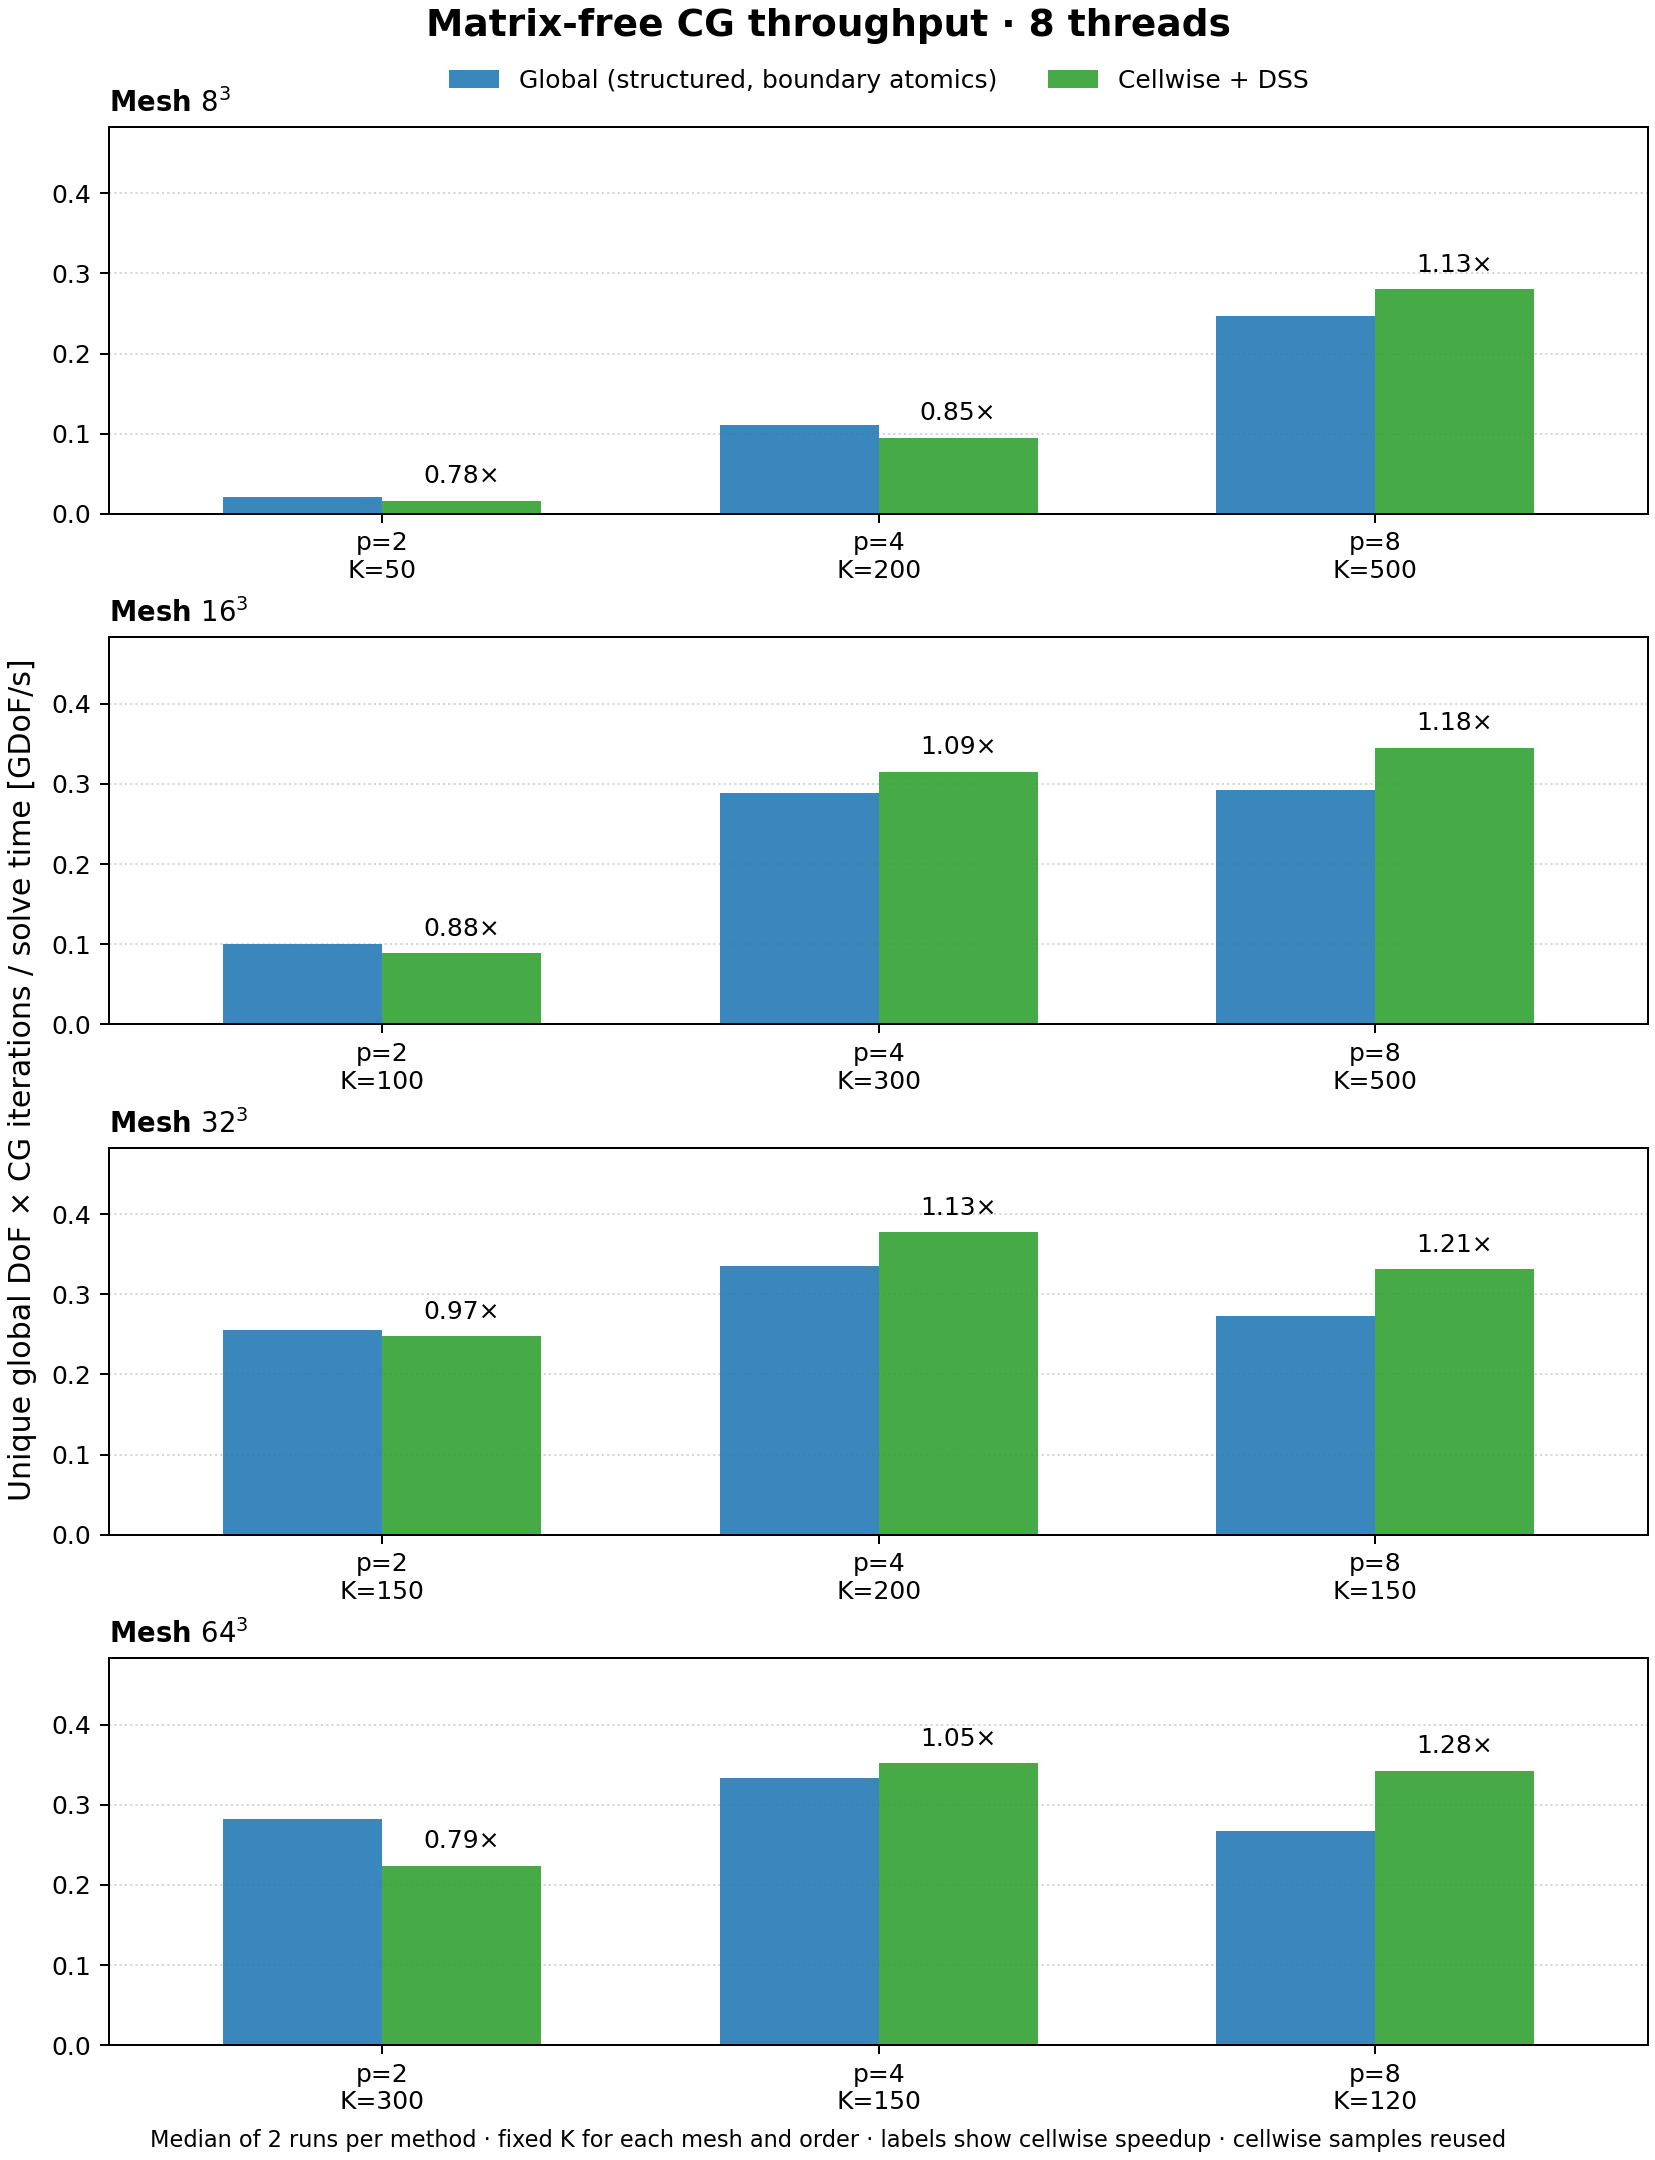
\includegraphics[width=\linewidth,trim=18bp 0 0 432bp,clip]{dss_bxyze_cg_fixed_budget_structured_boundary_released_throughput_t8.png}%
    \end{minipage}%
  }\par
  \vspace{0.13cm}
  {\centering\small\color{muted}Throughput $=\text{unique global DoFs}\times K/\text{solve time}$;
   $K$ is fixed per case.\par}
\end{frame}

\begin{frame}{Next work: semi-structured meshes on GPU}
  \vspace{-0.08cm}
  \begin{columns}[T,onlytextwidth]
    \begin{column}{0.57\textwidth}
      \centering
      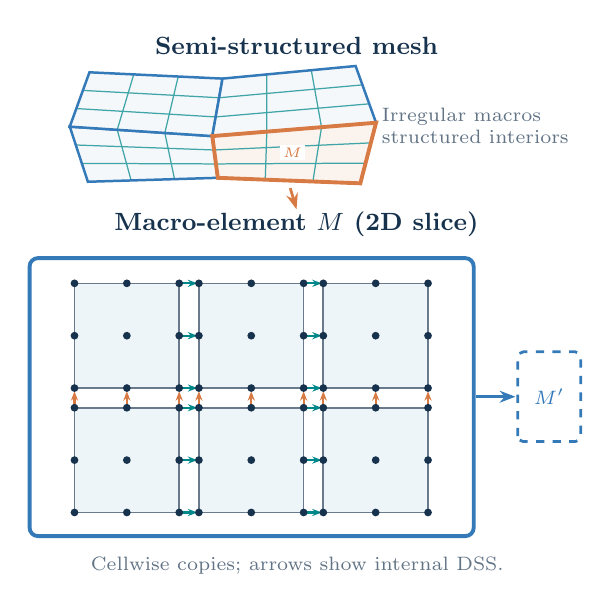
\begin{tikzpicture}[x=1cm,y=1cm]
        \node[font=\small\bfseries,text=ink] at (3.75,6.91)
          {Semi-structured mesh};
        \coordinate (A) at (1.10,5.18);
        \coordinate (B) at (2.75,5.23);
        \coordinate (C) at (4.56,5.16);
        \coordinate (D) at (0.87,5.88);
        \coordinate (E) at (2.68,5.76);
        \coordinate (F) at (4.76,5.93);
        \coordinate (G) at (1.12,6.57);
        \coordinate (H) at (2.81,6.49);
        \coordinate (I) at (4.50,6.65);
        \foreach \bl/\br/\tr/\tl/\shade in
          {A/B/E/D/blue!5,B/C/F/E/orange!9,D/E/H/G/blue!5,E/F/I/H/blue!5} {
          \fill[\shade] (\bl)--(\br)--(\tr)--(\tl)--cycle;
          \foreach \t in {0.333,0.667} {
            \draw[teal!75,line width=0.45pt]
              ($(\bl)!\t!(\br)$) -- ($(\tl)!\t!(\tr)$);
            \draw[teal!75,line width=0.45pt]
              ($(\bl)!\t!(\tl)$) -- ($(\br)!\t!(\tr)$);
          }
          \draw[blue,line width=0.9pt]
            (\bl)--(\br)--(\tr)--(\tl)--cycle;
        }
        \draw[orange,line width=1.4pt] (B)--(C)--(F)--(E)--cycle;
        \node[font=\tiny\bfseries,text=orange,fill=white,inner sep=1pt]
          at (3.70,5.55) {$M$};
        \node[font=\scriptsize,text=muted,align=left] at (6.02,5.89)
          {Irregular macros\\structured interiors};
        \draw[-{Stealth[length=2mm]},orange,line width=1pt]
          (3.67,5.10) -- (3.75,4.83);
        \node[font=\small\bfseries,text=ink] at (3.75,4.64)
          {Macro-element $M$ (2D slice)};
        \draw[blue,line width=1.4pt,rounded corners=3pt]
          (0.36,0.68) rectangle (6.00,4.21);
        \foreach \cx in {0,1,2} {
          \foreach \cy in {0,1} {
            \pgfmathsetmacro{\xx}{0.93+1.58*\cx}
            \pgfmathsetmacro{\yy}{0.98+1.58*\cy}
            \fill[pale] (\xx,\yy) rectangle ({\xx+1.33},{\yy+1.33});
            \draw[ink!65,line width=0.6pt]
              (\xx,\yy) rectangle ({\xx+1.33},{\yy+1.33});
          }
        }
        % Each arrow joins distinct cellwise copies of the same interface node.
        \foreach \cx in {0,1} {
          \foreach \cy in {0,1} {
            \foreach \j in {0,1,2} {
              \pgfmathsetmacro{\xa}{0.93+1.58*\cx+1.33}
              \pgfmathsetmacro{\xb}{0.93+1.58*(\cx+1)}
              \pgfmathsetmacro{\yn}{0.98+1.58*\cy+0.665*\j}
              \draw[-{Stealth[length=1.2mm,width=0.9mm]},teal,line width=0.75pt]
                ({\xa+0.02},\yn) -- ({\xb-0.02},\yn);
            }
          }
        }
        \foreach \cx in {0,1,2} {
          \foreach \i in {0,1,2} {
            \pgfmathsetmacro{\xn}{0.93+1.58*\cx+0.665*\i}
            \draw[-{Stealth[length=1.2mm,width=0.9mm]},orange,line width=0.75pt]
              (\xn,2.33) -- (\xn,2.52);
          }
        }
        \foreach \cx in {0,1,2} {
          \foreach \cy in {0,1} {
            \foreach \i in {0,1,2} {
              \foreach \j in {0,1,2} {
                \fill[ink] ({0.93+1.58*\cx+0.665*\i},
                            {0.98+1.58*\cy+0.665*\j}) circle (1.4pt);
              }
            }
          }
        }
        \draw[-{Stealth[length=2mm]},blue,line width=1.1pt]
          (6.03,2.45) -- (6.53,2.45);
        \draw[blue,dashed,line width=1pt,rounded corners=2pt]
          (6.56,1.88) rectangle (7.36,3.02);
        \node[font=\scriptsize,text=blue] at (6.96,2.45) {$M'$};
        \node[font=\scriptsize,text=muted] at (3.76,0.30)
          {Cellwise copies; arrows show internal DSS.};
      \end{tikzpicture}
    \end{column}
    \begin{column}{0.42\textwidth}
      {\small\bfseries Within each macro-element\par}
      \vspace{0.10cm}
      {\small
        \textbf{1. Gather} working values into GPU registers.\par
        \vspace{0.16cm}
        \textbf{2. Apply} the batched BXYZE cellwise operator.\par
        \vspace{0.16cm}
        \textbf{3. DSS} the duplicated nodes across structured subelements.\par
        \vspace{0.16cm}
        \textbf{4. Scatter} to distinct cellwise slots, without atomics inside $M$.\par
      }
      \vspace{0.23cm}
      {\setbeamercolor{block title}{fg=white,bg=orange}
       \setbeamercolor{block body}{fg=ink,bg=orange!8}
       \begin{block}{Between macro-elements}
         \small Inter-macro pass algorithm (\emph{Patrick's format}) to
         assemble the remaining shared interface nodes.
       \end{block}}
    \end{column}
  \end{columns}
\end{frame}

\end{document}
